\documentclass[11pt]{article}
\usepackage[T1]{fontenc}
\usepackage[margin=1in]{geometry}
\usepackage{amsmath,amssymb}
\usepackage{graphicx}
\usepackage{booktabs}
\usepackage{array}
\usepackage{xcolor}
\usepackage[colorlinks=true,linkcolor=blue!60!black,urlcolor=blue!60!black,
            citecolor=blue!60!black]{hyperref}
\usepackage[htt]{hyphenat}
\usepackage{microtype}
\emergencystretch=3em
\usepackage{listings}
\lstset{basicstyle=\ttfamily\footnotesize, backgroundcolor=\color{gray!8},
        frame=single, rulecolor=\color{gray!40}, breaklines=true,
        columns=fullflexible, keepspaces=true, showstringspaces=false}

\newcommand{\code}[1]{\texttt{#1}}
\newcommand{\file}[1]{\texttt{\small #1}}
\newcommand{\fn}[1]{\texttt{\small #1}}
\newcommand{\Om}{\Omega}

\title{Orbital Advection Across Azimuthal Level Jumps\\
       in the AthenaK Shearing Box\\[0.4em]
       \large \textsc{Validation Document}}
\author{\code{athenak-multigrid} tree, branch \code{fargo-amr}\\
        \small parent commit \code{d3edb948} (branch \code{dust-multigrid})}
\date{October 28, 2026}

\begin{document}
\maketitle

\begin{abstract}
\noindent
Orbital advection (FARGO) in the AthenaK shearing box now accepts $x_2$ neighbors one
level coarser or finer, so refinement may cover only part of the azimuth (method:
\file{fargo\_amr\_implementation.pdf}). This document records the tests. Every annular
and uniform configuration of the earlier test suite, hydro and MHD, is bit-identical to
the parent code. With the orbital-advection flux correction the remap conserves mass to
round-off across static and moving level jumps ($\sim5\times10^{-14}$ over hundreds of
steps; $10^{-7}$--$10^{-6}$ without it). Serial and 3-, 4- and 7-rank runs are
bit-identical, and the same tests run on an H200 GPU. A spatially uniform epicycle stays exactly uniform on a refined patch.
Vortical shearing waves on a static patch and under a moving box lie between the ring and
coarse-grid results, with no visible artifact at the level jumps. Swing amplification
with multigrid self-gravity on a patch moves the peak $0.60\%$ toward linear theory, and a
gravity-off control shows that gravity adds no deviation of its own. A timestep limit
lets a run proceed where the shift would otherwise exceed the neighbor's rows. For MHD
(branch \code{fargo-amr-mhd}) orbital advection now runs on refined meshes, rings and
partial-$x_2$ patches alike: the remap's EMFs are corrected at level jumps, which keeps the
two copies of every shared face equal to round-off ($10^{-2}$ apart without it), and the
refined-mesh field error of the magnetized swing (13--22\% without orbital advection) is
gone: refined runs follow their uniform twins to 1--3\% and linear theory better than the
uniform runs. Pushed into collapse ($4\pi G\rho_0 = 6$) with a Jeans-length criterion
(16 cells, three levels), patches and rings give the same collapse --- the same site, the
same time, winding waves within $0.012$ of each other where refinement itself moves them by
$0.13$ --- with $8.6$ times fewer MeshBlock-cycles for patches; both collapse earlier than a
uniform $256^2$ run, because between the crests the criterion leaves the box at the
$128^2$ root. Magnetized ($\beta = 8$), the refined runs collapse at the centre, $1.2$
time units before a uniform $256^2$ run, which collapses on the shear-periodic $x_1$
boundary, where the mesh policy forbids refinement. AMR regrids with two or more levels leave the two copies of shared faces
$10^{-7}$--$10^{-3}$ apart, with or without orbital advection; like the $\nabla\!\cdot\!B$
jumps at derefinement ($10^{-13}$--$10^{-12}$ per event next to fine $x_2$ neighbours), this
is a pre-existing AthenaK defect, documented here. The production test
--- SC14 clump-following AMR with and without rings --- is still to be run.
\end{abstract}

\tableofcontents
\newpage

%=========================================================================================
\section{Test ladder}
\label{sec:ladder}
All runs are on a Mac (Apple Silicon, serial build and Open MPI build), October 28, 2026,
except those of \S\ref{sec:gpu} and \S\ref{sec:clump} (one H200 GPU).
Run directories are in \file{validation/run/fargo\_amr/}; its \file{README.md} lists
the command for each one. ``Patch'' means a refined region that covers only part of
$x_2$, so it has $x_2$ level jumps; ``ring'' means the old annular configuration.

\begin{center}
\small
\begin{tabular}{@{}>{\raggedright\arraybackslash}p{4.6cm}>{\raggedright\arraybackslash}p{5.6cm}p{4.0cm}@{}}
\toprule
Test & What it probes & Result \\
\midrule
Regression (\S\ref{sec:regression}) & same-level path unchanged & bit-identical \\
Epicycle on a patch (\S\ref{sec:epicycle}) & buffers, indices, prolongation & exact \\
Conservation (\S\ref{sec:conservation}) & flux correction, static and AMR &
  $5\times10^{-14}$ \\
MPI (\S\ref{sec:mpi}) & per-sub-face messages and tags & bit-identical \\
Vortical shearing wave (\S\ref{sec:shwave}) & structure through level jumps &
  between ring and coarse \\
Swing with gravity (\S\ref{sec:swing}) & multigrid at $x_2$ level jumps & $+0.60\%$
  toward theory \\
Timestep limit (\S\ref{sec:dtlimit}) & large shifts & runs, conserves \\
MHD on rings (\S\ref{sec:mhd}) & orbital EMF correction, field error &
  faces to $10^{-15}$; 1--3\% \\
MHD across $x_2$ jumps (\S\ref{sec:mhdB}) & $B_1$, $B_3$ rows across levels &
  faces to $10^{-15}$; 1--3\% \\
Swing to collapse (\S\ref{sec:clump}) & Jeans-criterion AMR, patches vs rings &
  same collapse, 8.6$\times$ fewer blocks \\
SC14 production (\S\ref{sec:open}) & cost & not yet run \\
\bottomrule
\end{tabular}
\end{center}

%=========================================================================================
\section{Regression: nothing changes where nothing jumps}
\label{sec:regression}
On a same-level face the new code performs the same arithmetic as before, only with a
different buffer layout and depth. Each input below was run with a build of the parent
commit and with the new build, and the binary dumps (the data after the parameter header,
which differs by the added input line) and history files compared byte by byte. All are
\textbf{bit-identical}:

\begin{center}
\small
\begin{tabular}{@{}>{\raggedright\arraybackslash}p{7.6cm}p{6.6cm}@{}}
\toprule
Input (\file{inputs/shearing\_box/}) & Configuration \\
\midrule
\file{epicycle\_smr\_ring} & level-1 ring, 1 orbit \\
\file{epicycle\_amr\_ring}, \file{epicycle\_amr\_ring2} & moving ring, 1 and 2 levels,
  incl.\ block create/destroy sequence \\
\file{hydro\_incompress\_shwave\_smr\_ring\{,2\}} & ring, 1 and 2 levels \\
\file{hydro\_incompress\_shwave\_amr\_ring} & moving ring \\
\file{epicycle}, \file{hydro\_incompress\_shwave}, \file{hydro\_compress\_shwave} &
  uniform mesh (VTK dumps for the shwaves) \\
\file{mhd\_compress\_shwave} & uniform mesh, MHD with orbital advection \\
\bottomrule
\end{tabular}
\end{center}

\noindent
The AMR ring inputs were run with \code{oa\_annular = true}, which they need for the
ring-wise flag synchronization (now off by default). The new orbital-advection timestep
limit does not bind in any of them.

%=========================================================================================
\section{The epicycle on a patch}
\label{sec:epicycle}
\file{epicycle\_smr\_ypatch.athinput}: $20\times20\times1$ box, $128^2\times4$ root
cells, $32^2\times4$ blocks; the level-1 region covers $|x|, |y| < 5$, two of the four
block rows in $y$, so four $x_2$ faces are level jumps. The \code{ipert=1} epicycle is
spatially uniform at all times, so any error in buffer layout, indexing or prolongation
appears as $O(1)$ structure. After one orbit (365 steps):
\begin{itemize}\itemsep2pt
\item density, all velocity components and the internal energy are uniform to the last
      digit of the single-precision output in every one of the 44 blocks;
\item every history column matches the ring run (\file{epicycle\_smr\_ring}), and the
      mass does not change;
\item on 4 MPI ranks every dump is bit-identical to the serial run.
\end{itemize}

%=========================================================================================
\section{Exact conservation}
\label{sec:conservation}
A uniform field cannot show a conservation error, and the vortical shwave of
\S\ref{sec:shwave} has amplitude $10^{-4}$ and constant density. The conservation test
is therefore the compressible shwave (\file{hydro\_compress\_shwave\_smr}, isothermal,
HLLE, PLM) at amplitude $0.1$ on a $4\times4$ box, $128^2\times4$ root cells, $32^2\times4$
blocks, with a level-1 patch over $|x|, |y| < 1$. The $x_1$ boundaries are plain
\emph{periodic}: the shear-periodic remap at the $x_1$ faces is itself conservative only to
$\sim10^{-8}$ and would hide the effect. Only the hydro update and the orbital remap then
move mass. The moving-box variant uses the AMR criterion of the implementation document
with $x_c = 0.9\sin t$, $y_c = 0.8\sin 2t + t$ and half-widths $0.3$.

\begin{center}
\small
\begin{tabular}{@{}lcc@{}}
\toprule
maximum $|M(t) - M(0)|/M(0)$ & flux correction on & off \\
\midrule
static patch, $t = 0$--$2$ (453 steps)                                 & $5.2\times10^{-14}$ & $1.8\times10^{-7}$ \\
moving box (AMR), $t = 0$--$4$ (899 steps; 98 blocks created, 84 destroyed) & $5.7\times10^{-14}$ & $1.0\times10^{-6}$ \\
static patch, shear-periodic $x_1$                                    & $3.8\times10^{-9}$ & $1.1\times10^{-7}$ \\
\bottomrule
\end{tabular}
\end{center}

\noindent
With the correction the remap is conservative to round-off, through regridding too
(Fig.~\ref{fig:conservation}); the total $y$-momentum stays at $3\times10^{-16}$ against
$5\times10^{-7}$ without. With shear-periodic $x_1$ boundaries the correction still
removes most of the drift; the remaining $4\times10^{-9}$ is the boundary remap.

\begin{figure}[htb]
  \centering
  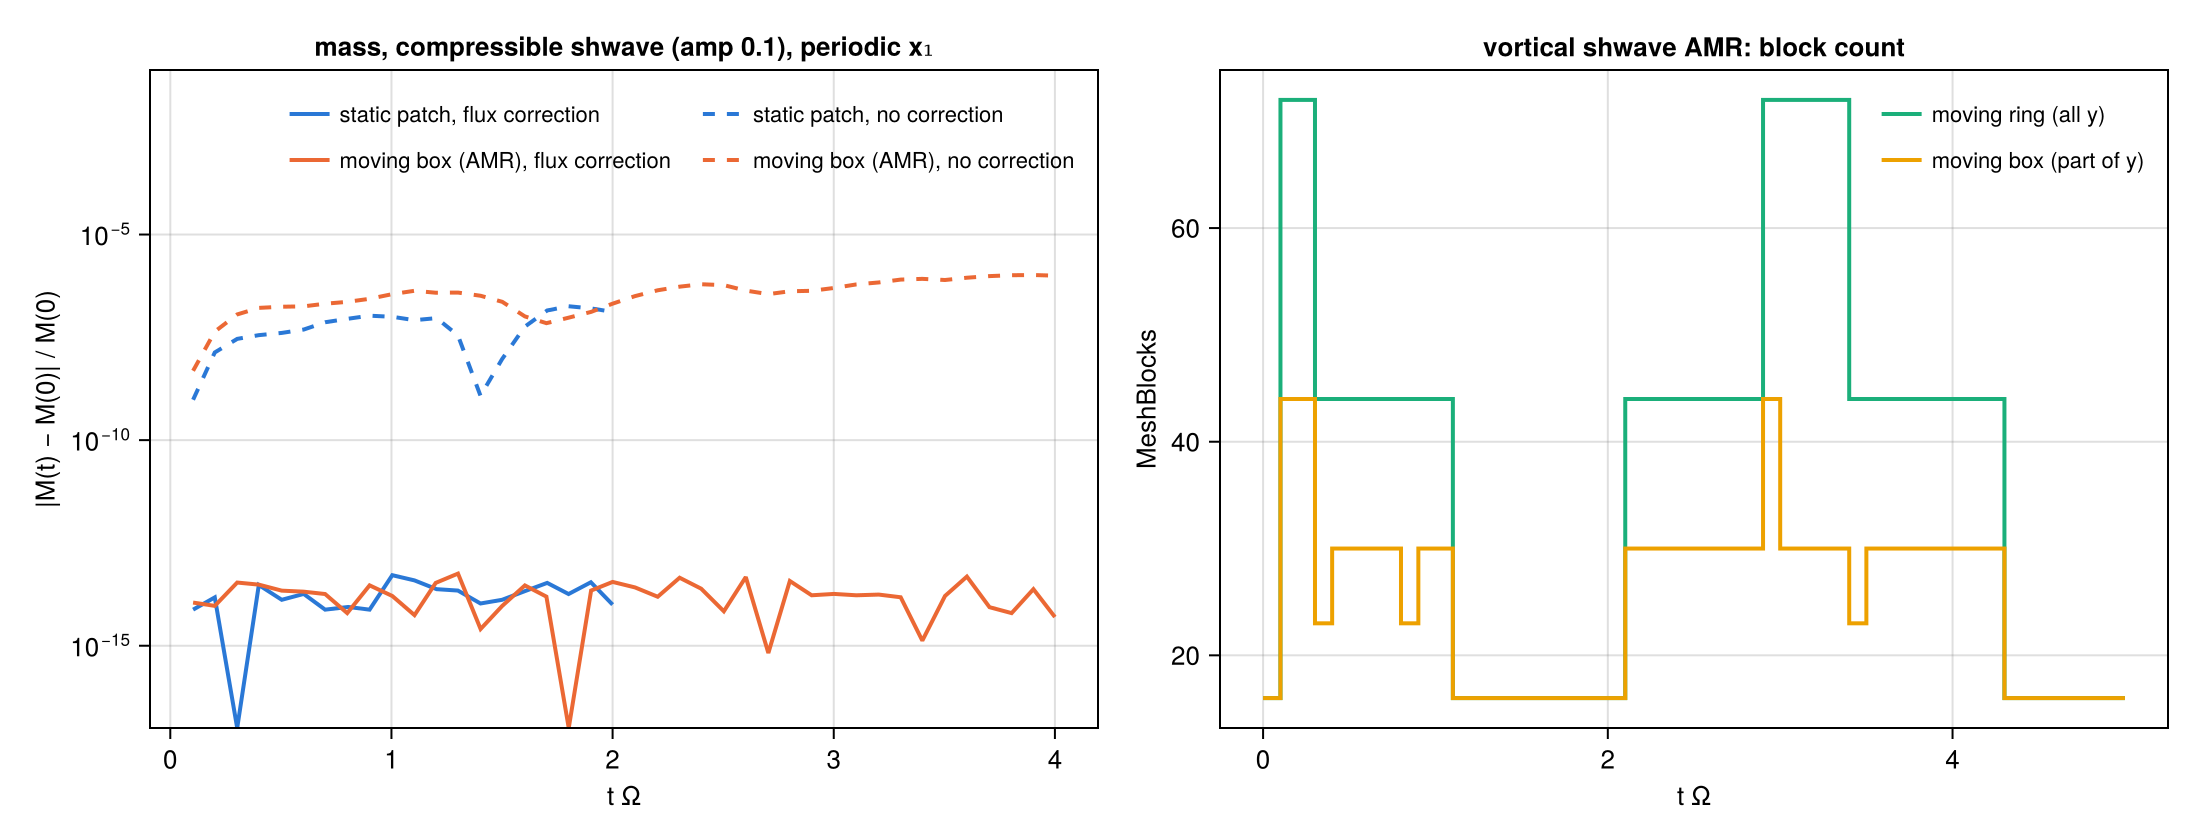
\includegraphics[width=\textwidth]{figures/fargo_amr_conservation.png}
  \caption{Left: relative mass drift of the compressible shwave (amplitude 0.1, periodic
  $x_1$) on a static patch (blue) and under a moving box with AMR (orange), with (solid)
  and without (dashed) the orbital-advection flux correction. Right: MeshBlock count of
  the vortical-shwave AMR runs of \S\ref{sec:shwave} --- the moving box refines part of
  the ring's blocks. Script \file{figures/plot\_fargo\_amr\_tests.jl}.}
  \label{fig:conservation}
\end{figure}

%=========================================================================================
\section{MPI}
\label{sec:mpi}
The conservation runs (static patch and moving box) were repeated on 3, 4 and 7 ranks.
All binary dumps are bit-identical to the serial runs. The history files differ only in
the volume sums, by the MPI reduction order: $\le 6.5\times10^{-13}$ on a mass of 16, and
$\sim10^{-15}$ in momenta whose value is itself round-off. Mass is conserved to
$1\times10^{-14}$ on every rank count. The vortical-shwave moving box on 4 ranks is
likewise bit-identical to the serial run in all 51 dumps.

%=========================================================================================
\section{Vortical shearing wave through static and moving level jumps}
\label{sec:shwave}
The Johnson \& Gammie (2005) vortical shwave (\code{ipert=2}, isothermal, PPM;
$64^2\times4$ root cells on $0.5\times0.5$, $16^2\times4$ blocks, $t = 0$--$5$) on five
meshes, compared with a uniform $128^2$ run as the reference:

\begin{center}
\small
\begin{tabular}{@{}lccc@{}}
\toprule
run & refined region (level 1) & peak $x$-KE vs $128^2$ & $\max|\Delta{\rm KE}_x|/{\rm peak}$ \\
\midrule
uniform $64^2$                         & ---                            & $-4.5\%$  & $1.1\times10^{-1}$ \\
ring, static                           & $|x|<0.125$, all $y$           & $-7.9\%$  & $8.2\times10^{-2}$ \\
patch, static                          & $|x|,|y|<0.125$                & $-8.1\%$  & $9.3\times10^{-2}$ \\
moving ring, AMR                       & $x_c = 0.2\sin t$              & $-12.2\%$ & $1.3\times10^{-1}$ \\
moving box, AMR                        & $+\;y_c = 0.15\sin t + 0.1t$   & $-11.9\%$ & $1.3\times10^{-1}$ \\
\bottomrule
\end{tabular}
\end{center}

\noindent
Inputs: \file{hydro\_incompress\_shwave\{,\_smr\_ring,\_smr\_ypatch,\_amr\_ring,\_amr\_box\}};
all history output at full precision (\code{output1/data\_format=\%.15e}). The patch lies
between the ring and the coarse grid in the history error, and the moving box matches
the moving ring (the box creates and destroys 77 blocks, the ring 112;
Fig.~\ref{fig:conservation}, right). The peak error of the ring is larger than that of the
coarse grid; this is a property of the ring runs, not of this work.

Figure~\ref{fig:errmap} maps the $v_x$ error against the $128^2$ run. Inside the static
patch the error is larger than inside the ring at $t = 1$: the wave reaches the fine
region after crossing coarse cells in $y$, while in the ring it never leaves the fine
grid. At the $x_2$ level jumps the error bands run straight across, with no stripes or
kinks. Averaged over the refined $x_1$ columns of the patch, the error next to the jumps
lies between those of the fine interior and the coarse rows ($t = 1$:
$9.1$, $4.9$ and $11\times10^{-2}$ of $\max|v_x|$; at $t = 2.5$ the three agree to
$10\%$).

\begin{figure}[htb]
  \centering
  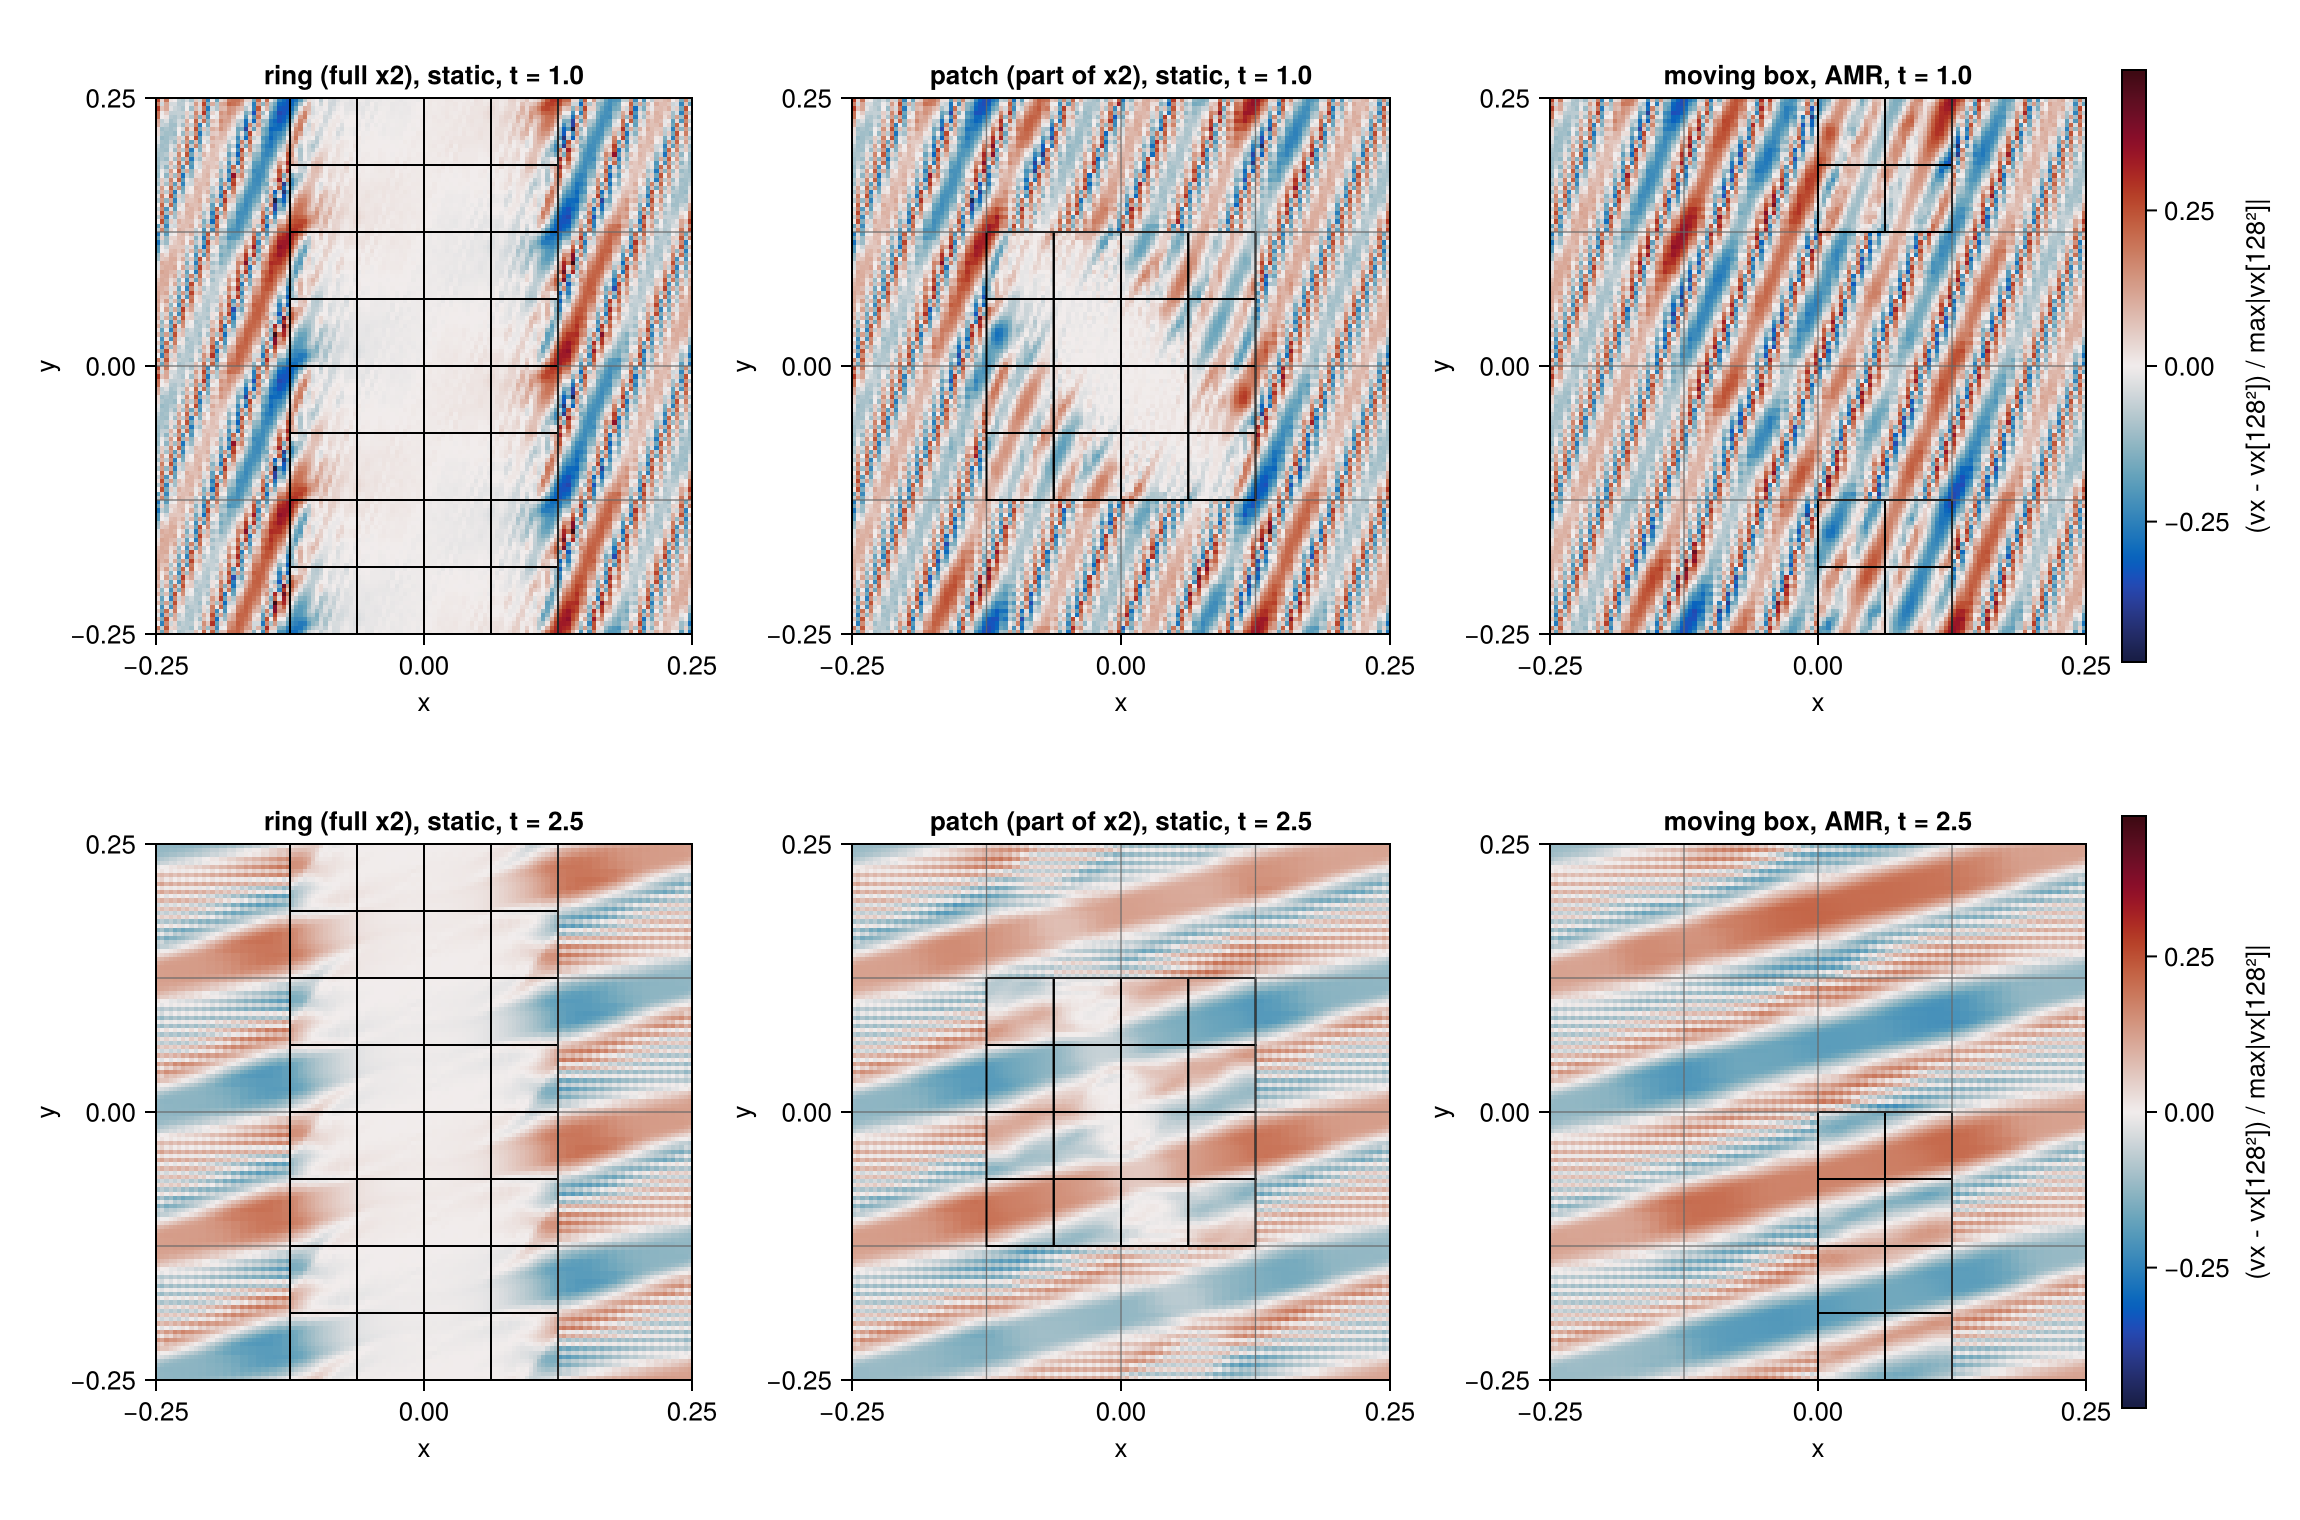
\includegraphics[width=\textwidth]{figures/fargo_amr_shwave_err.png}
  \caption{$v_x$ error of the vortical shwave against a uniform $128^2$ run, normalized to
  $\max|v_x|$, averaged over $z$, shown at the finest resolution (coarse cells repeated),
  at $t = 1$ (top) and $t = 2.5$ (bottom). Left: ring. Middle: static patch, $x_2$ level
  jumps at $y = \pm0.125$. Right: moving box (AMR). Black: refined blocks; grey: root
  blocks. The checkerboard in coarse regions is the coarse cells against the fine
  reference. Script \file{figures/plot\_fargo\_amr\_shwave.jl}.}
  \label{fig:errmap}
\end{figure}

The planned twin without orbital advection is not available for patches: with
\code{orbital\_advection = false}, the patch mesh collapses at the first step
($\Delta t \to 10^{-45}$) \emph{in the parent code as well}, with or without
\code{prolong\_primitives}. The ring mesh runs. This is a separate, pre-existing problem
(\S\ref{sec:open}).

%=========================================================================================
\section{Swing amplification with multigrid gravity on a patch}
\label{sec:swing}
\file{tests/swing\_selfgrav\_smr\_ypatch.athinput} is the swing test of
\file{multigrid\_sb\_validation.pdf} (Phase 2a: $2\pi\times2\pi\times\pi/4$,
$128^2\times16$ root cells, $16^3$ blocks, $4\pi G\rho_0 = 1.9$, a leading wave with
$k_x/k_y = -6$) with the level-1 region cut to the middle four of eight block rows in $y$
(six of eight columns in $x$, as for the ring). The $x_2$ faces at $y = \pm\pi/2$ are then
level jumps for orbital advection and for the multigrid octets. The ring and uniform runs
were repeated with the new code.

\begin{center}
\small
\begin{tabular}{@{}lccc@{}}
\toprule
run & peak $d_{\cos}/A$ & peak time & $\max|d_{\sin}|/A$ \\
\midrule
uniform, multigrid        & $-3.511418$ & $7.804$ & $7.3\times10^{-14}$ \\
ring                      & $-3.583481$ & $7.804$ & $1.3\times10^{-13}$ \\
patch                     & $-3.532422$ & $7.804$ & $6.1\times10^{-13}$ \\
\bottomrule
\end{tabular}
\end{center}

\noindent
The uniform and ring runs reproduce the Phase-2a values to the last digit. The patch
moves the peak $0.60\%$ toward the converged answer (linear theory 3.605), under a
third of the ring's $2.05\%$, with half the ring's refined area; the phase lock stays at
machine level. The gravity-off control (\code{hydro\_srcterms/self\_gravity=false})
attributes the shift as in Phase 2a: the patch-vs-uniform deviation is larger without
gravity ($5.8\times10^{-2}$ maximum, peak $+1.11\%$) than with it ($3.6\times10^{-2}$,
$+0.60\%$), so multigrid gravity across the $x_2$ level jumps adds no deviation of its own
(Fig.~\ref{fig:swing}).

\begin{figure}[htb]
  \centering
  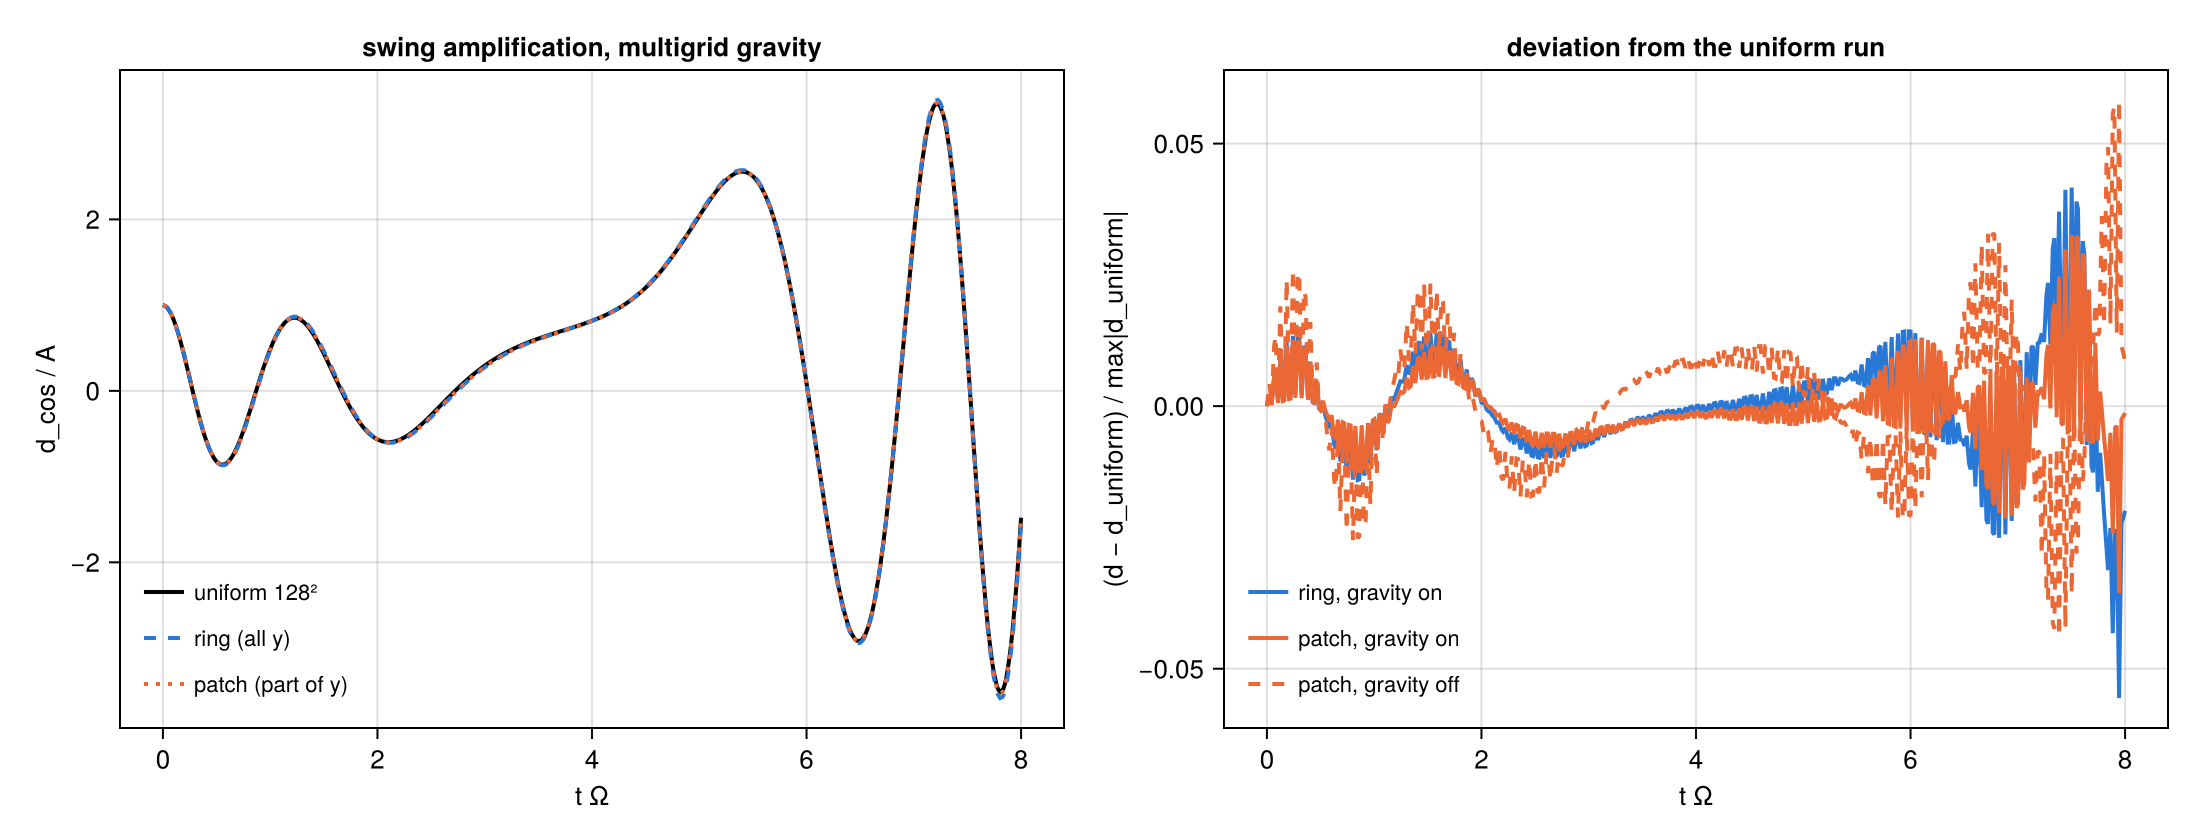
\includegraphics[width=\textwidth]{figures/fargo_amr_swing.png}
  \caption{Swing amplification with multigrid self-gravity. Left: projection of the
  density onto the shearing wave, $d_{\cos}/A$, for the uniform, ring and patch meshes
  (indistinguishable at this scale). Right: deviation from the uniform run, with gravity
  (solid) and, for the patch, without (dashed). The fast
  oscillation of the deviations is present in the ring run as well. Script
  \file{figures/plot\_fargo\_amr\_tests.jl}.}
  \label{fig:swing}
\end{figure}

%=========================================================================================
\section{The timestep limit}
\label{sec:dtlimit}
A cold variant of the static-patch conservation test (sound speed $0.05$, amplitude
$10^{-3}$) lets the hydro timestep grow until the shift at $|x| = 2$ would be 8 cells
against 6 available rows. The build without the limit stops at the first step with the
guard's message. With it, $\Delta t$ is held at
$0.999\,(6-2)\,\Delta x_2/(q\Om\max|x|) = 0.0416$, exactly the predicted value; the run
reaches $t = 8$ (193 steps) and conserves mass to $8\times10^{-14}$.

%=========================================================================================
\section{MHD with orbital advection on refined meshes}
\label{sec:mhd}
Branch \code{fargo-amr-mhd}, in two steps. First, MHD with orbital advection on refined
meshes whose refinement comes in complete $x_2$ rings (\code{oa\_annular = true}; the
subsections up to the magnetized swing); then across $x_2$ level jumps
(\S\ref{sec:mhdB}). The effective EMFs of
the face-field remap are corrected at level jumps like the stage EMFs (implementation
document, section ``Magnetic fields: MHD on rings''). Before this, MHD $+$ orbital advection $+$ refinement was a
fatal error, and the refined MHD shearing boxes of \file{multigrid\_sb\_validation.pdf}
(Phase 4) ran without orbital advection, where the field perturbation of the magnetized
swing is $13$--$22\%$ off.

\subsection{Regression}
Uniform MHD with orbital advection (\file{mhd\_compress\_shwave}) is bit-identical to the
parent code in the history and all VTK dumps: without refinement the remap's EMFs are not
corrected and the arithmetic is unchanged.

\subsection{The refined-mesh field error disappears with orbital advection}
The three-minute reproducer of the Phase-4 field error
(\file{inputs/tests/swing\_mhd\_repro.athinput}: $64^2\times4$ root cells, $8^2\times4$
blocks, $B_0 = 1$ along $y$, $\beta = 1.2$, static level-1 ring $|x| < \pi/4$), run with
and without orbital advection. It is a magnetized shearing wave without self-gravity: the
Phase-4 work found the error with and without gravity and dropped it to isolate the
defect. The swing amplification with self-gravity follows in \S\ref{sec:mhdgrav}
(Fig.~\ref{fig:mhd}). Deviation over $t \le 6$, on common
times:

\begin{center}
\small
\begin{tabular}{@{}lccc@{}}
\toprule
& \multicolumn{2}{c}{vs linear theory} & ring vs uniform twin \\
run & $\delta$ & $c_y$ & $c_y$ \\
\midrule
uniform, no orbital advection   & 0.068 & 0.075 & --- \\
ring, no orbital advection      & 0.075 & 0.226 & 0.220 \\
uniform, orbital advection      & 0.091 & 0.106 & --- \\
ring, orbital advection         & 0.062 & 0.074 & 0.033 \\
\bottomrule
\end{tabular}
\end{center}

\noindent
With orbital advection the ring is closer to linear theory than its uniform twin, as
refinement should be, and within $3.3\%$ of it ($\delta$: $3.0\%$), where the same ring
without orbital advection is $22\%$ off. The two uniform runs
agree with each other to $3\%$. So the Phase-4 defect needs the background shear flow
carried in the state across the level interfaces; with orbital advection the state holds
only the perturbation and the defect does not arise. (Comparing the twins row by row of
the history, as \file{repro.py} did, is wrong when one run's step exceeds the history
interval --- the uniform run with orbital advection takes $\Delta t = 0.021$ against an
output interval of 0.02 --- and gave a spurious $52\%$; \file{repro.py} now interpolates to
common times.)

\begin{figure}[htb]
  \centering
  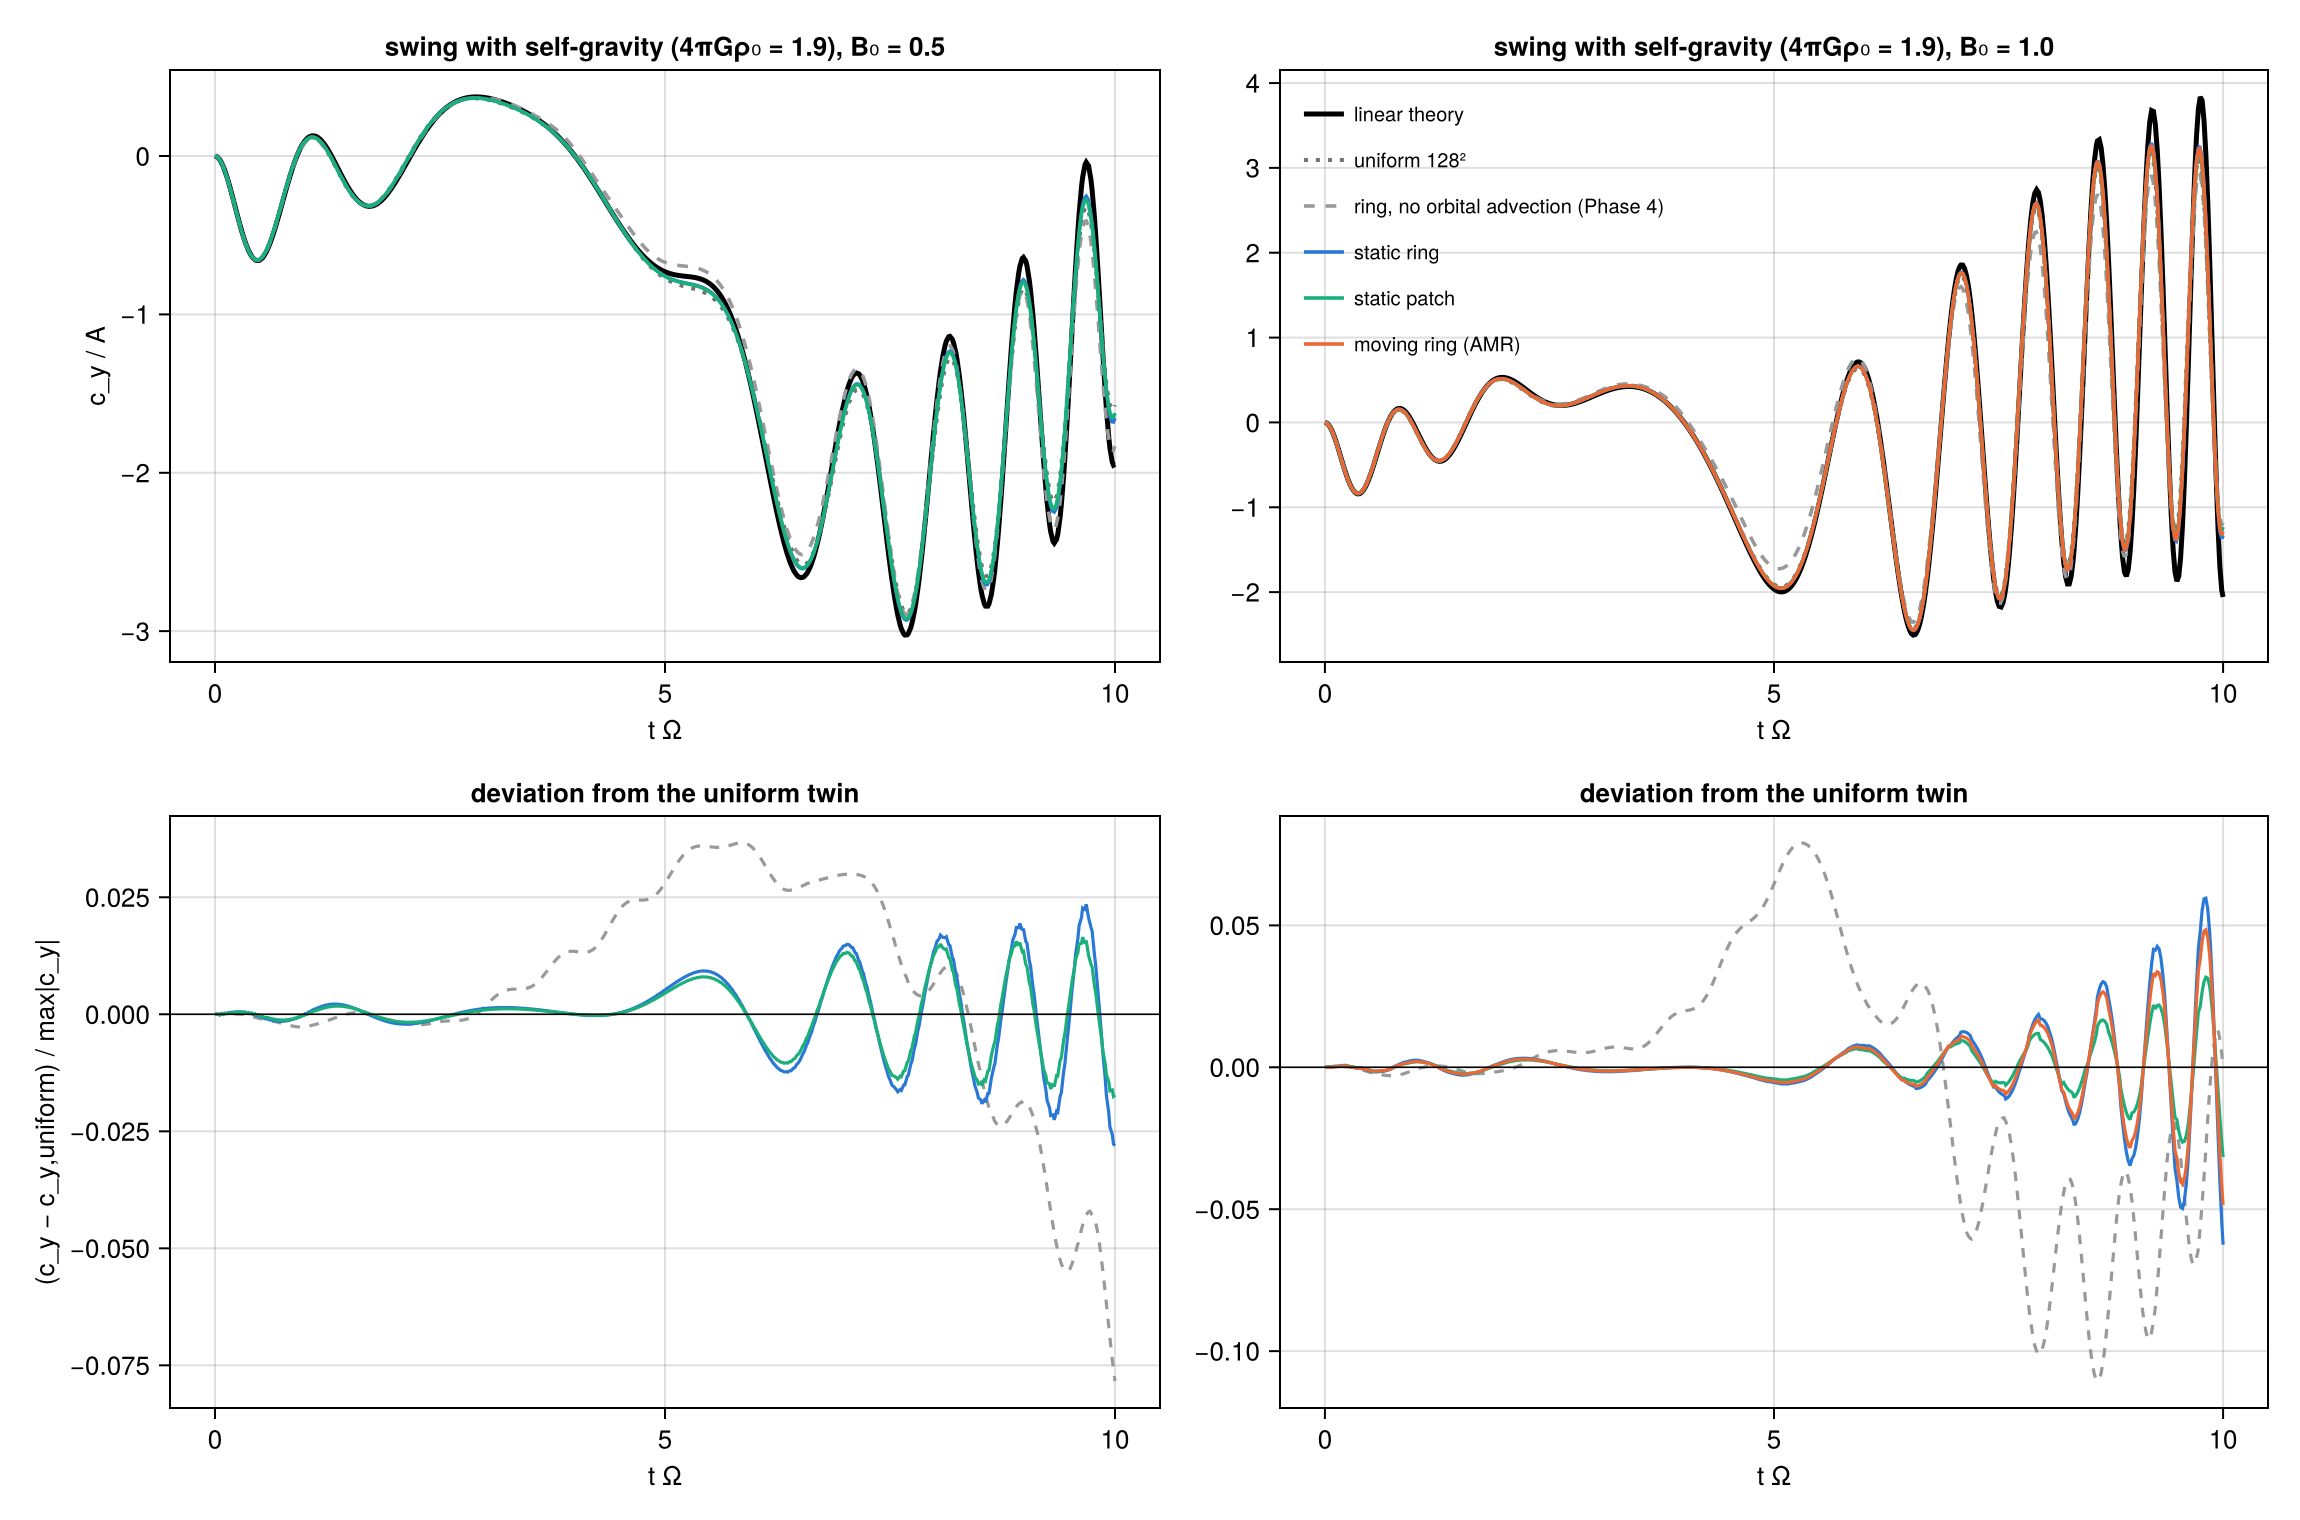
\includegraphics[width=\textwidth]{figures/fargo_amr_mhd.png}
  \caption{Magnetized swing amplification with self-gravity
  (\file{inputs/tests/swing\_mhd.athinput}: $128^2\times16$ root, multigrid gravity with
  $4\pi G\rho_0 = 1.9$, amplitude $10^{-4}$), $B_0 = 0.5$ (left) and $1.0$ (right). Top:
  azimuthal field perturbation $c_y$ against linear theory (black; \file{swing\_ode.py},
  7-point Laplacian at the root spacing) for the uniform run and, with orbital advection,
  a static ring, a static patch ($|y| < \pi/2$, \S\ref{sec:mhdB}) and a moving ring (AMR);
  dashed, the Phase-4 ring without orbital advection. Bottom: deviation from the uniform
  twin in the same frame (orbital advection or not), normalized by the twin's maximum
  $|c_y|$ over $t \le 10$ (the tables use $t \le 6$). Script
  \file{figures/plot\_fargo\_amr\_mhd.jl}.}
  \label{fig:mhd}
\end{figure}

\subsection{Shared faces stay consistent}
The history columns \code{bmis}/\code{bnrm} measure how far the coarse copy of each face
shared with a finer block is from the mean of the fine copies:

\begin{center}
\small
\begin{tabular}{@{}lccc@{}}
\toprule
& \multicolumn{2}{c}{copy mismatch $/\,|B_n|$} & \\
mesh & EMF correction off & on & $\max|\nabla\!\cdot\!B|/|B|$ \\
\midrule
ring (level jumps at $x_1$ faces)                         & $\sim 10^{-2}$ (up to 0.7) & $\sim10^{-15}$ & $4\times10^{-15}$ \\
ring $+$ half-height in $z$ ($x_1$ and $x_3$ jumps)        & median $1.8\times10^{-2}$ & $\sim10^{-15}$ & $3\times10^{-15}$ \\
moving ring, AMR (280 blocks created, 224 destroyed)       & median $3\times10^{-3}$ & $\sim10^{-15}$ & $5\times10^{-15}$ \\
ring without orbital advection (stage EMFs only)           & \multicolumn{2}{c}{$\sim10^{-15}$} & $4\times10^{-15}$ \\
\bottomrule
\end{tabular}
\end{center}

\noindent
Without the correction the two copies drift apart by about $1\%$ of the field (the ratio
peaks where $B_n$ passes through zero); each block stays divergence-free, which is why the
history's $\nabla\!\cdot\!B$ does not see it. With it they agree to round-off, as the
stage's own EMF correction keeps them without orbital advection
(Fig.~\ref{fig:mhdfaces}). The effect on the smooth swing wave is small ($2$--$4\times10^{-4}$ in $\delta$ and
$c_y$), but a shared face with two different values is a monopole of the composite mesh.
On 4 MPI ranks every field dump of the $x_3$-jump and AMR runs is bit-identical to the
serial run.

\begin{figure}[htb]
  \centering
  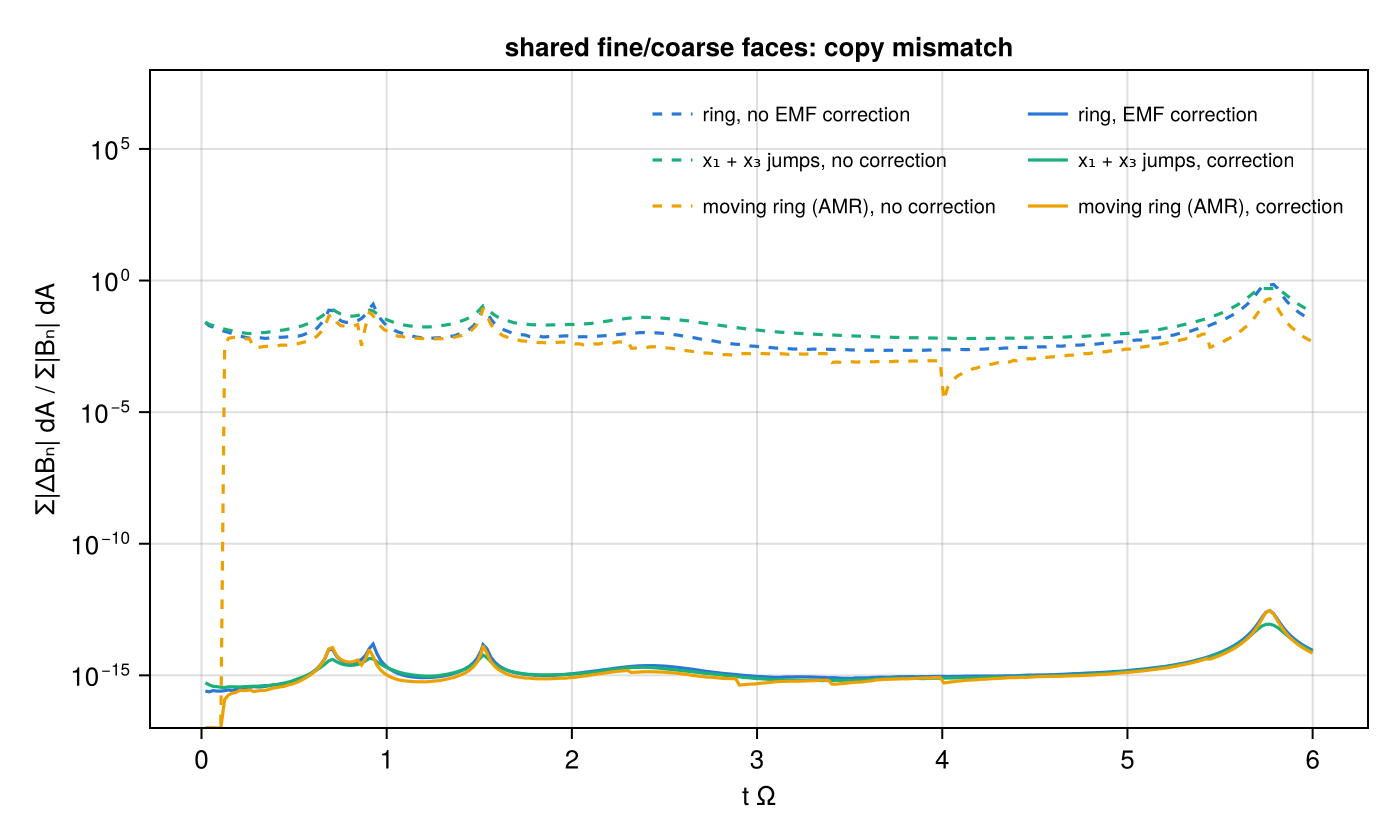
\includegraphics[width=0.62\textwidth]{figures/fargo_amr_mhd_faces.png}
  \caption{Mismatch of the two copies of the faces shared by fine and coarse blocks, with
  (solid) and without (dashed) the EMF correction of the face-field remap, in the
  gravity-free reproducer: ring, ring with $x_3$ level jumps, moving ring (AMR). Script
  \file{figures/plot\_fargo\_amr\_mhd.jl}.}
  \label{fig:mhdfaces}
\end{figure}

\subsection{Magnetized swing amplification with gravity}
\label{sec:mhdgrav}
The full Phase-4 test (\file{inputs/tests/swing\_mhd.athinput}: $128^2\times16$ root
cells, $16^3$ blocks, multigrid gravity with $4\pi G\rho_0 = 1.9$, HLLD, PLM) on the
two-column ring and the moving ring of Phase 4, now with orbital advection, against the
uniform runs with orbital advection (\code{uF\_b*}). Deviation from the uniform twin over
$t \le 6$, with the Phase-4 values without orbital advection for comparison:

\begin{center}
\small
\begin{tabular}{@{}lcccc@{}}
\toprule
& \multicolumn{2}{c}{orbital advection (this work)} &
  \multicolumn{2}{c}{without (Phase 4)} \\
case & $\delta$ & $c_y$ & $\delta$ & $c_y$ \\
\midrule
static ring, $B_0 = 0.5$   & 0.035 & 0.017 & 0.025 & 0.071 \\
static ring, $B_0 = 1.0$   & 0.014 & 0.014 & 0.039 & 0.133 \\
moving ring, $B_0 = 1.0$   & 0.013 & 0.013 & 0.040 & 0.150 \\
\bottomrule
\end{tabular}
\end{center}

\noindent
Figure~\ref{fig:mhd} shows $c_y$ against linear theory and the deviation from the
uniform twin, together with the patch runs of \S\ref{sec:mhdB}. With orbital advection the
refined runs follow their uniform twins to $1$--$4\%$ in
$\delta$ and $1$--$2\%$ in $c_y$, against $7$--$15\%$ in $c_y$ without it. Against linear
theory they are closer than the uniform runs, as refinement should be: $c_y$ is off by
$3.2\%$ and $2.7\%$ on the static rings ($B_0 = 0.5$, $1.0$) and $2.9\%$ on the moving ring,
against $4.9\%$ and $4.0\%$ for the uniform runs. The shared faces stay consistent to
round-off (copy mismatch $\le 10^{-12}$ of $|B_n|$) and $\max|\nabla\!\cdot\!B|/|B| \le
7\times10^{-15}$. The static rings (176 MeshBlocks) ran to $t = 10$; to $t \le 8$ their
$c_y$ deviation is $1.7\%$ and $2.6\%$. The moving ring (64--176 MeshBlocks; 448 created,
392 destroyed) also ran to $t = 10$: $1.9\%$ and $2.3\%$ to $t \le 8$, with
$\nabla\!\cdot\!B \le 5\times10^{-15}$ throughout. All on 3 MPI ranks; inputs and runs in
\file{validation/run/fargo\_amr/mhd/swing/}.

So with orbital advection, refined MHD shearing boxes are validated on rings, with and
without self-gravity; the refined-mesh field error of Phase 4 remains a property of the
full-shear-flow frame.

\subsection{Across \texorpdfstring{$x_2$}{x2} level jumps}
\label{sec:mhdB}
In the second step the face-field remap takes $x_2$ neighbours one level coarser or finer
(implementation document), and MHD with orbital advection follows the hydro policy:
\code{oa\_annular} is optional.

\paragraph{Regression.} Uniform MHD with orbital advection is still bit-identical to the
parent code, and the ring, $x_3$-jump and moving-ring reproducer runs of the first step are
bit-identical to their first-step results: the same-level path is unchanged.

\paragraph{Reproducer on a patch.} The reproducer with the ring cut to four of eight block
rows in $y$ ($|x| < \pi/4$, $|y| < \pi/2$; 120 MeshBlocks), and with a moving box under AMR
(the moving ring of the first step with an $x_2$ window $y_c = \sin t + 0.5\,t$, half-width
0.6; 64--106 MeshBlocks, 147 created, 126 destroyed):

\begin{center}
\small
\begin{tabular}{@{}lcccc@{}}
\toprule
& \multicolumn{2}{c}{vs uniform twin} & copy mismatch $/\,|B_n|$ & \\
mesh & $\delta$ & $c_y$ & correction on / off & $\max|\nabla\!\cdot\!B|/|B|$ \\
\midrule
ring (first step)            & 0.030 & 0.033 & $10^{-15}$ / $10^{-2}$ & $4\times10^{-15}$ \\
static patch ($x_2$ jumps)   & 0.025 & 0.026 & $2\times10^{-15}$ / $6\times10^{-7}$ & $4\times10^{-15}$ \\
moving box, AMR              & 0.023 & 0.023 & $10^{-15}$ / $2\times10^{-7}$ & $4\times10^{-12}$ (see below) \\
\bottomrule
\end{tabular}
\end{center}

\noindent
On the patch the field perturbation follows its uniform twin as closely as on the ring, and
every shared face, now including the $x_2$ faces, stays consistent to round-off. (Without the
correction the normalized mismatch is smaller than on the ring only because the $x_2$ faces
add their normal field $B_y \approx B_0 = 1$ to the normalization; the absolute mismatch is
of the same order.) On 4 MPI ranks every field dump of both runs is bit-identical to the
serial run.

\paragraph{A pre-existing $\nabla\!\cdot\!B$ defect at AMR derefinement.} In the moving-box run
$|\nabla\!\cdot\!B|/|B|$ grows in steps, $10^{-13}$ to $5\times10^{-12}$, at the regrid events
where blocks are \emph{derefined}, and stays constant in between (so the remap and its
correction conserve it). Two controls place it outside this work: the same moving box with
$q = 0$ (the remap then shifts nothing) and with $q = 0$ and orbital advection off give the
same jumps at the same events ($3.9\times10^{-13}$ at $t = 0.28$, $7.1\times10^{-12}$ by
$t = 3$). The moving ring of the first step derefines too (392 blocks destroyed in the full
swing run) and stays at $5\times10^{-15}$; a box adds fine neighbours across $x_2$ faces and
$x_1x_2$ edges to a derefined block. The suspect is AthenaK's post-AMR face-field handling
(\fn{MeshRefinement::RepairAMRFC}, which recomputes the interior faces of created \emph{and}
derefined blocks, or the face ownership of the receives at those neighbours). It is small
now but accumulates with every derefinement; it is left for a separate fix.

\paragraph{Magnetized swing with gravity on a patch.} The full test of
\S\ref{sec:mhd} (multigrid gravity, $128^2\times16$, 3 MPI ranks) with the two-column ring cut
to half the azimuth ($|y| < \pi/2$):

\begin{center}
\small
\begin{tabular}{@{}lcccc@{}}
\toprule
& \multicolumn{2}{c}{vs uniform twin, $t \le 6$} & vs theory, $t \le 6$ & \\
case & $\delta$ & $c_y$ & $c_y$ & $\max|\nabla\!\cdot\!B|/|B|$ \\
\midrule
patch, $B_0 = 0.5$ & 0.030 & 0.015 & 0.035 & $5\times10^{-15}$ \\
patch, $B_0 = 1.0$ & 0.012 & 0.011 & 0.030 & $6\times10^{-15}$ \\
ring, $B_0 = 0.5$ (above) & 0.035 & 0.017 & 0.032 & $6\times10^{-15}$ \\
ring, $B_0 = 1.0$ (above) & 0.014 & 0.014 & 0.027 & $7\times10^{-15}$ \\
\bottomrule
\end{tabular}
\end{center}

\noindent
The patch (120 MeshBlocks) follows its uniform twin as closely as the ring, $1$--$3\%$ in
$\delta$ and $c_y$, also to $t \le 8$ ($1.4\%$, $1.7\%$ at $B_0 = 1.0$), and linear theory
better than the uniform runs ($c_y$: $3.5\%$ and $3.0\%$ against $4.9\%$ and $4.0\%$). Shared
faces agree to $5\times10^{-15}$ of $|B_n|$, and $\nabla\!\cdot\!B$ stays at round-off. Runs in
\file{validation/run/fargo\_amr/mhd/swing/} (\code{ypF\_b*}, input \file{ypatch.athinput}) and
\file{mhd/stepB/} (reproducer).

%=========================================================================================
\section{GPU}
\label{sec:gpu}
The same inputs on one NVIDIA H200 (h-gpu; CUDA 13.3, Kokkos Hopper build, no MPI), October
28, 2026. The CUDA compiler found one defect the CPU build accepts: an extended device
lambda in a private member function (\fn{OrbitalAdvectionFC::UpdateB}), now public. Then
all thirteen runs (seven hydro, six MHD; 31~s in total) ran to the same cycle counts as on
the CPU:

\begin{center}
\small
\begin{tabular}{@{}>{\raggedright\arraybackslash}p{5.4cm}>{\centering\arraybackslash}p{2.6cm}>{\raggedright\arraybackslash}p{6.0cm}@{}}
\toprule
runs & GPU vs CPU (max over $t$) & checks on the GPU \\
\midrule
hydro: conservation, $\Delta t$ limit, epicycle, shwave patch and box & $\le 8\times10^{-13}$ &
  mass $\le 10^{-14}$ with correction, $1.8\times10^{-7}$ without \\
MHD: ring, ring without correction, patch, uniform & $\le 2\times10^{-12}$ &
  face mismatch $\le 3\times10^{-13}$, $\nabla\!\cdot\!B \le 4\times10^{-15}$ \\
MHD: $x_3$ jumps, moving box & $\le 7\times10^{-9}$ &
  face mismatch $\le 10^{-13}$; box $\nabla\!\cdot\!B$ $2\times10^{-12}$ (\S\ref{sec:mhdB}) \\
\bottomrule
\end{tabular}
\end{center}

\noindent
(GPU vs CPU: physical history columns --- mass, energies, wave projections --- relative to
their maxima.) Repeated GPU runs of the two last cases are bit-identical, so the larger
GPU--CPU difference there is round-off growing differently (limiter branches at
near-zero differences), not a race. Runs in \file{h-gpu:/data/limjay/runs/fargo\_amr\_gpu/},
scripts \file{build\_cuda.slurm}, \file{run\_tests.slurm}.

%=========================================================================================
\section{Nonlinear swing to collapse}
\label{sec:clump}
The swing tests so far are linear. This section pushes the swing of
\file{multigrid\_sb\_validation.pdf} (\S13, Figs.~9--11 there) into collapse, with the
refinement now free to follow the clump as a patch. Setup
(\file{inputs/tests/swing\_selfgrav\_clump\_jeans.athinput}): $2\pi\times2\pi\times\pi/4$,
$128^2\times16$ root cells, $16^3$ blocks, isothermal, HLLE, PLM, multigrid gravity with
$4\pi G\rho_0 = 6$, a leading wave $k_x/k_y = -6$ of amplitude $0.2$, orbital advection on,
to $t = 10$. At these parameters the uniform run of \S13 fragments at $t \approx 4.5$ and
forms a bound clump near $t \approx 9$. In \S13 the zoom was one level, triggered by density
($\rho > 2$), and had to come in complete $x_2$ rings. Here it is the Jeans criterion of the
implementation document (\fn{SwingJeansRefine}): a block is refined where
$\lambda_J = 2\pi c_s/(4\pi G\rho)^{1/2}$ is shorter than 16 of its cells, up to three
levels, and derefined where $\lambda_J$ exceeds 40 cells everywhere in it. $\lambda_J$ is
52 root cells at $\rho_0$, so the levels switch on at $\rho = 10.7$, 43 and 171, and level 3
keeps $\lambda_J \geq 16$ cells up to $\rho = 683$. The 128$^2$ Truelove limit ($\lambda_J
= 4$ cells) is 171. All runs on one H200 (h-gpu), October 28, 2026.

\paragraph{Hydro.} Uniform $128^2$, the same with $x_2$ rings (\code{oa\_annular = true}),
with patches (\code{oa\_annular = false}), uniform $256^2$, and a marginal case
($4\pi G = 5$, amplitude 0.05, patches) that should not collapse:

\begin{center}
\small
\begin{tabular}{@{}lccccc@{}}
\toprule
run & peak $\rho/\rho_0$ (at $t$) & first $\rho > 100$ & max blocks & MeshBlock-cycles & wall time \\
\midrule
uniform $128^2$            & 203 (9.40) & 9.30 & 64      & $1.2\times10^5$ & 1.6 min \\
uniform $256^2$            & 40.4 (10.0) & ---  & 512     & $1.5\times10^6$ & 5.4 min \\
AMR, rings                 & 286 (9.50) & 9.20 & 4768    & $1.3\times10^7$ & 57 min \\
AMR, patches               & 377 (10.0) & 9.15 & 610     & $1.5\times10^6$ & 23 min \\
marginal, patches          & 2.70 (5.65) & ---  & 64      & $5.6\times10^4$ & 0.8 min \\
\bottomrule
\end{tabular}
\end{center}

\noindent
The uniform $128^2$ run reproduces \S13 on the GPU: peak $203.28\rho_0$ at $t = 9.40$, the
CPU value to the printed digits.

\emph{Patches and rings give the same collapse.} Both refined runs step through the same
first crest (peak $25.62\rho_0$ at $t = 4.65$, level 1 only), cross $\rho = 10.7$ again at
$t = 8.20$/$8.25$ and $\rho = 100$ at $9.15$/$9.20$, and collapse at the same site
(Fig.~\ref{fig:clump_maps}). Their winding-wave amplitudes $d_{\cos}/A$ differ by at most
$0.012$ up to $t = 7$ and $0.08$ up to $t = 8$, against $0.13$ between either and the uniform
run already at $t \le 7$ (Fig.~\ref{fig:clump}, middle): the choice of patch or ring is ten
times smaller than the effect of refinement itself, until the collapse turns chaotic
($t \gtrsim 8.5$; afterwards peak densities differ by up to a factor 2 between any two runs,
as the clump oscillates).

\emph{Refinement moves the clump to where the resolved runs of \S13 put it.} The uniform
$128^2$ run ends with one clump at the box centre ($131\rho_0$ at $(0.02, -0.02)$, peak 203
at $t = 9.4$, above its Truelove limit). Both refined runs collapse instead at $y = \pm\pi$, as a
pair of knots related by the inversion symmetry of the initial wave (patches at $t = 9.5$:
$161.6\rho_0$ at $(-0.26, -2.65)$ and $(0.26, 2.65)$), one of which wins by $t = 10$
($369\rho_0$ on patches, $206\rho_0$ on rings, in the midplane). That is the site of the
dominant knot of the uniform $256^2$ multigrid run and of its FFT twin in \S13, which
identified the $128^2$ central clump as the under-resolved outlier. The uniform $256^2$ run has not collapsed by $t = 10$: it holds a thin
filament along $y$ at $x \approx 0$, densest near $y = \pm\pi$ ($40.4\rho_0$ at
$(\mp0.01, \mp2.88)$, the \S13 value), where its extension to $t = 14$ in \S13 forms the
dominant knot.

\emph{But refinement does not fix the clock.} The $256^2$ run collapses about one time unit
later: at $t = 8.5$ its peak is $1.9\rho_0$, against $20$--$22\rho_0$ in the refined runs and
$8.4\rho_0$ in the uniform $128^2$ run. Between the crests ($t = 5.2$ to $8.2$) every block of
the refined runs is back at level 0 --- the gas is at $\rho \lesssim 4$, where $\lambda_J$
is 26 root cells or more --- so for those three time units they are $128^2$ runs. The
winding wave says the same: against the $256^2$ run, $d_{\cos}/A$ of the refined runs is
off by $0.14$--$0.19$ up to $t = 7$ (the uniform $128^2$ run by $0.27$--$0.31$), and all
three part from it at $t \approx 8$. The Jeans criterion at 16 cells resolves gravity; it
does not resolve the hydrodynamics of the wound-up crests at $\rho \approx 2$--$4$, which
still differ between $128^2$ and $256^2$. A converged collapse time needs a finer root grid
or a criterion that also refines the crests; neither was run.

\emph{The clump stays resolved.} The peak stays below 683, so level 3 keeps
$\lambda_J \ge 16$ cells to the end; the uniform $128^2$ run overshoots its Truelove limit
(203 against 171).

\emph{Cost.} Rings refine the clump's $x_1$ columns at all $y$: at $t = 9.5$, 4096 level-3
blocks (eight rings of 512) to hold a clump a few level-3 blocks across. Patches need 610 at
most, a factor 8.6 fewer MeshBlock-cycles over the run. On the GPU the wall time drops only
by 2.5: a 600-block mesh does not fill an H200, and the AMR machinery (regridding every
five cycles, multigrid across levels, the orbital-advection messages per sub-face) costs
per block. Per MeshBlock-cycle the patch run takes 0.90~ms, the ring run 0.26~ms, the
uniform $256^2$ run 0.21~ms --- which therefore finishes in a quarter of the patch run's
wall time with the same number of MeshBlock-cycles. On CPUs, where the cost follows the
block count, patches gain the full factor over rings.

\emph{The marginal case.} At $4\pi G = 5$, amplitude 0.05, the crest peaks at $2.70\rho_0$ ($t = 5.65$)
and re-expands, as in \S13; $\lambda_J$ never falls below 16 cells, no block is refined,
and the run is the uniform run (the same peak to seven digits as the CPU run of \S13).

\begin{figure}[htb]
  \centering
  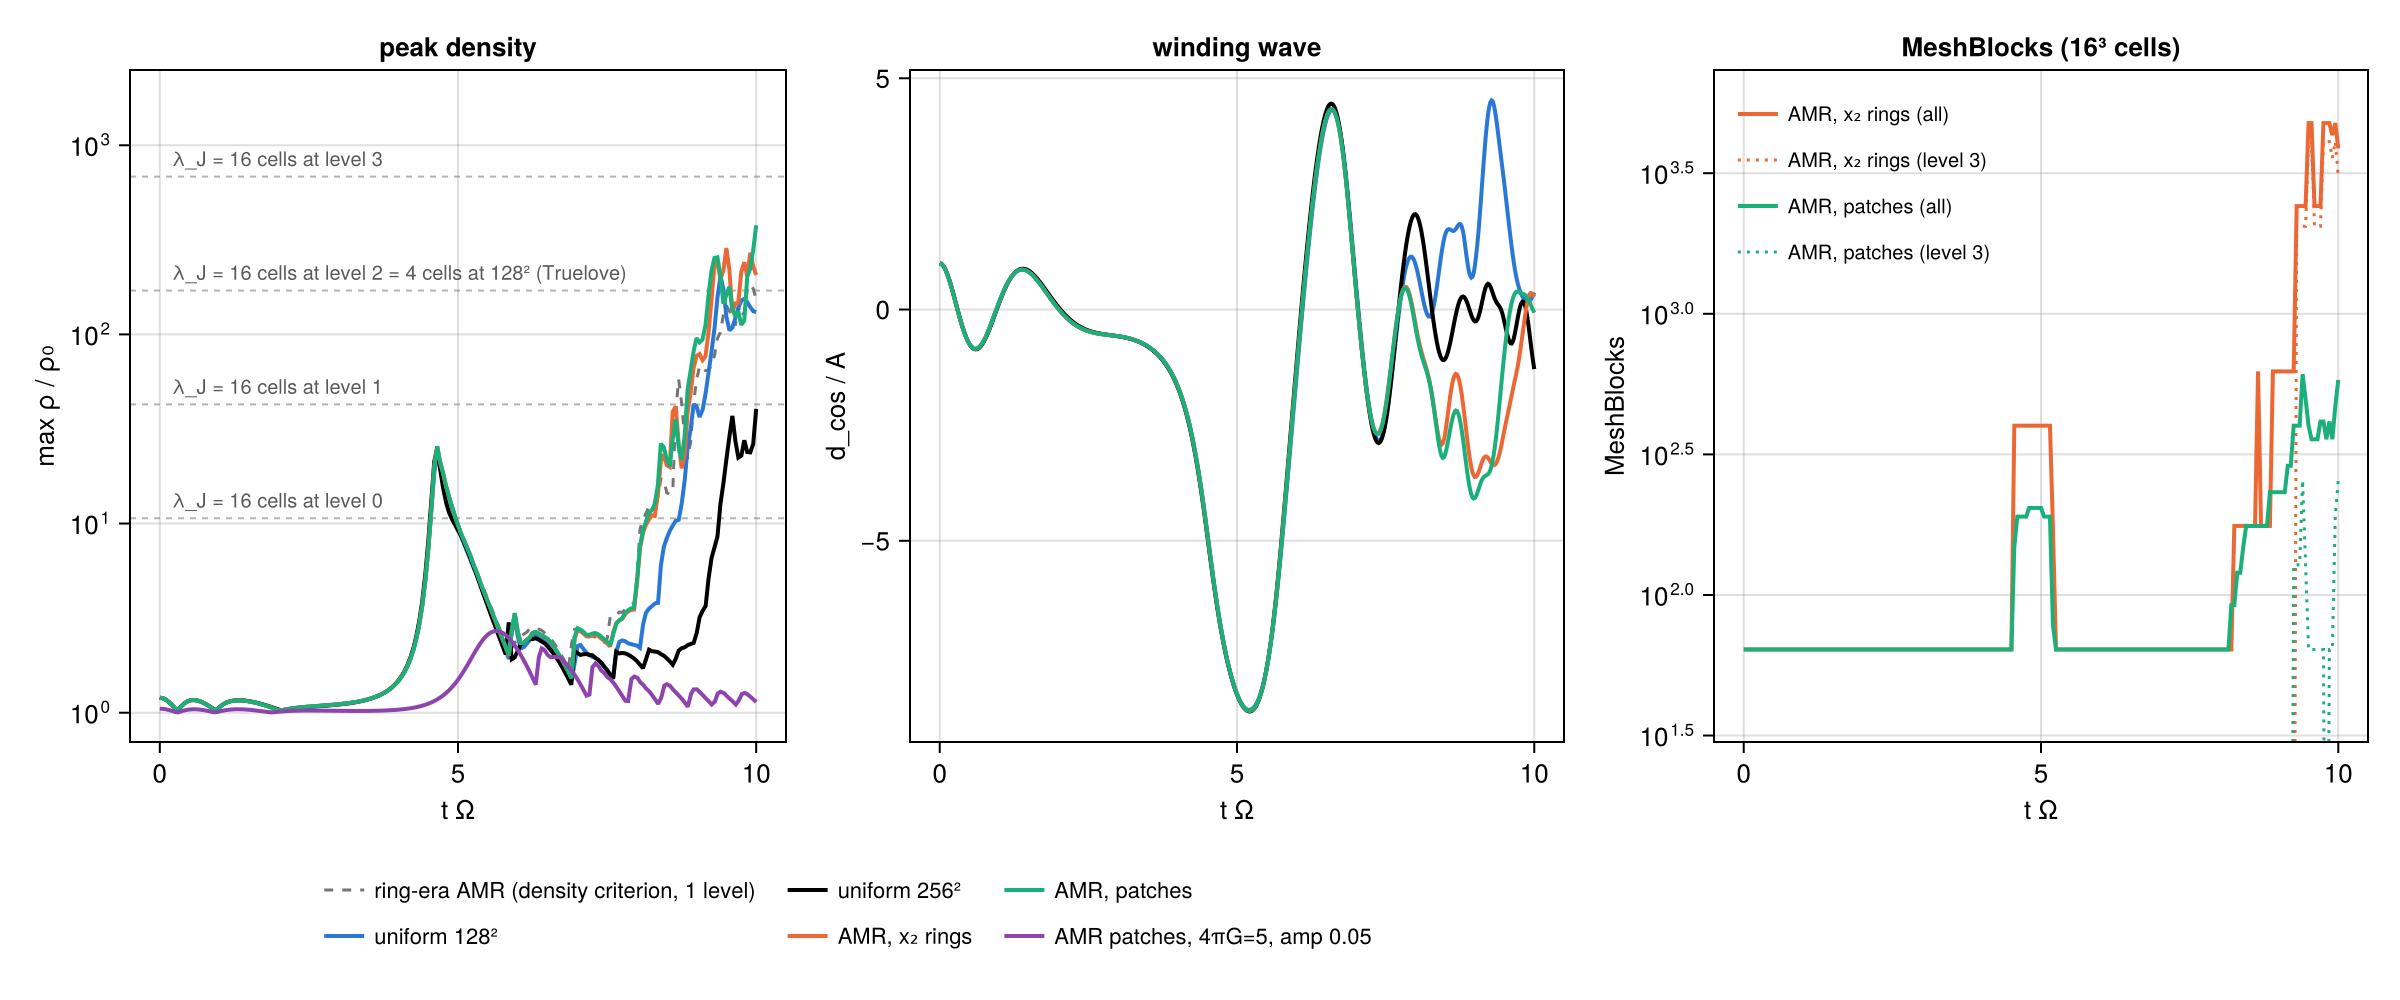
\includegraphics[width=\textwidth]{figures/fargo_amr_clump.png}
  \caption{Nonlinear swing to collapse, hydro ($4\pi G = 6$, amplitude 0.2). Left: peak
  density, with the densities at which $\lambda_J$ falls to 16 cells of levels 0--3 (the
  refinement thresholds), the ring-era run of \S13 (one level, density criterion) and
  the marginal case.
  Middle: winding-wave amplitude; the refined runs part from the uniform $128^2$ run
  after the first crest ($t \approx 5$) and from each other at $t \approx 8.5$. Right: MeshBlock count, total
  (solid) and level 3 (dotted). Script \file{figures/plot\_fargo\_amr\_clump.jl}.}
  \label{fig:clump}
\end{figure}

\begin{figure}[htb]
  \centering
  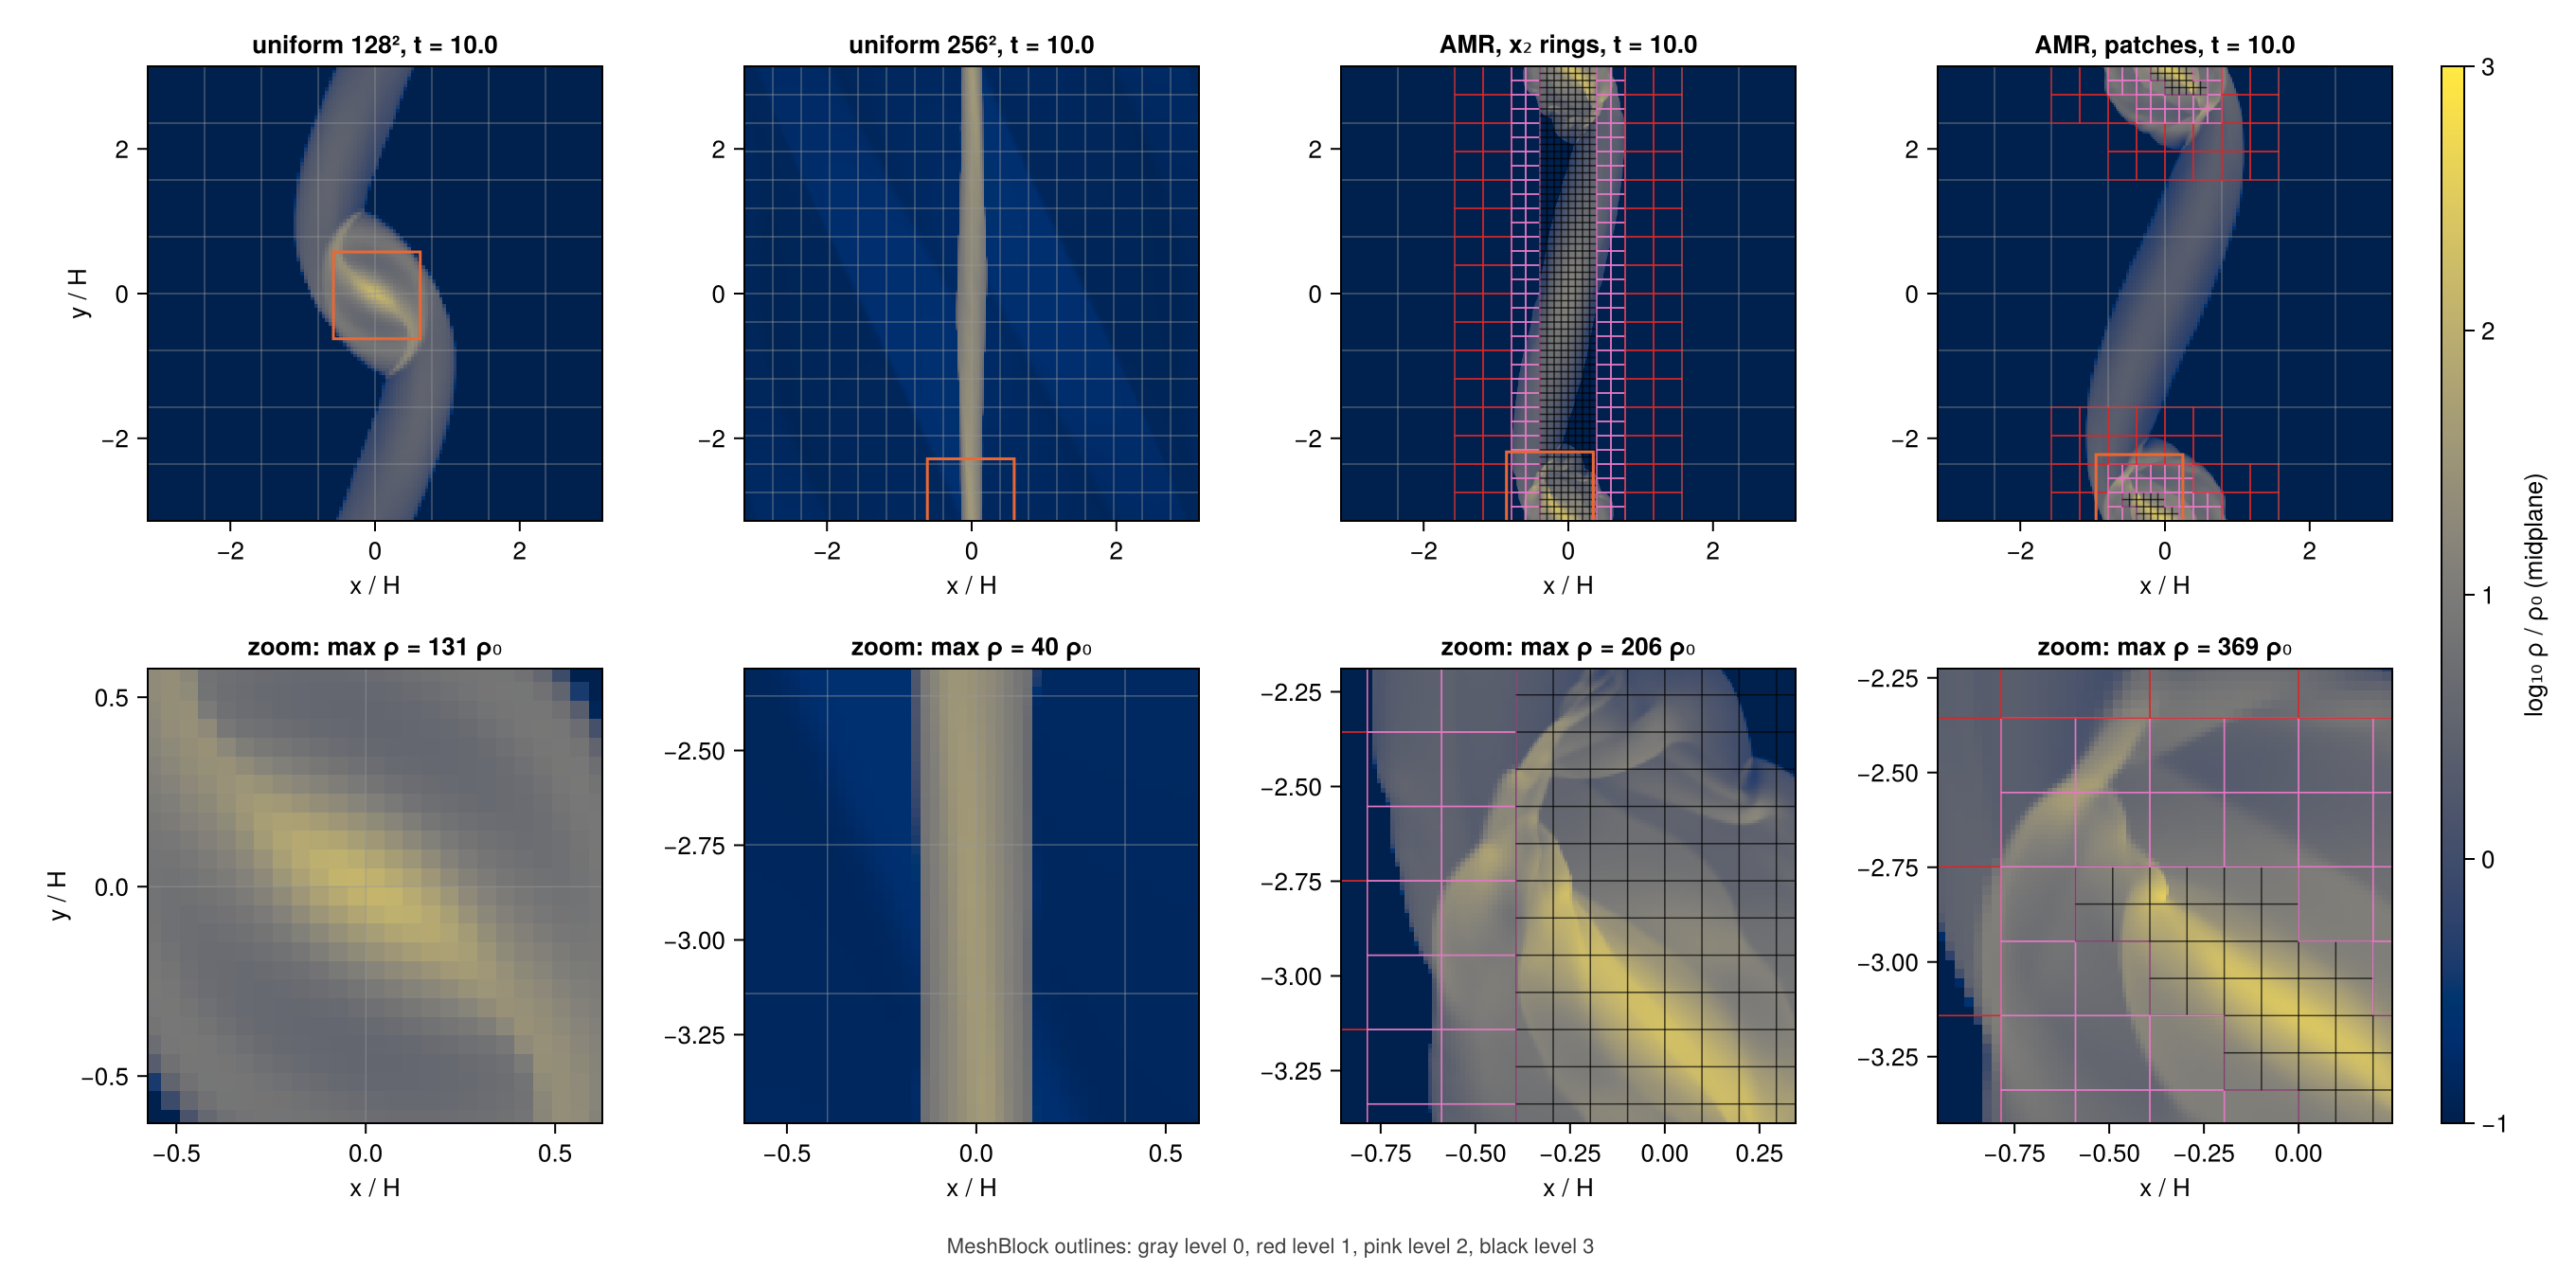
\includegraphics[width=\textwidth]{figures/fargo_amr_clump_maps.png}
  \caption{Midplane density at $t = 10$ with MeshBlock outlines (top) and a
  $1.2\times1.2$ zoom centred on each run's densest cell (bottom; the box is periodic in
  $y$, so the zoom may cross $y = \pm\pi$). The refined runs collapse at $y = \pm\pi$, where the
  $256^2$ filament is densest; the uniform $128^2$ run at the centre.}
  \label{fig:clump_maps}
\end{figure}

\paragraph{MHD.} The same with a uniform field along $y$
(\file{inputs/tests/swing\_mhd\_clump\_jeans.athinput}; isothermal HLLE --- isothermal HLLD
is unstable at $\beta \lesssim 1$ --- and the thermal Jeans length, so the criterion ignores
magnetic support): $B_0 = 0.5$ ($\beta = 8$) on the three $128^2$ meshes and uniform
$256^2$ (to $t = 12$), and $B_0 = 0.25$ uniform and on patches:

\begin{center}
\small
\begin{tabular}{@{}lcccccc@{}}
\toprule
run & first crest & $\rho > 100$ & $\rho > 683$ & max $\rho/\rho_0$ & MeshBlock-cycles & wall time \\
\midrule
uniform, $B_0 = 0.5$   & 38.0 (4.45) & ---  & ---  & 38          & $9.5\times10^4$ & 1.4 min \\
rings, $B_0 = 0.5$     & 36.8 (4.45) & 9.70 & 9.90 & $1.4\times10^4$ & $7.3\times10^6$ & 34 min \\
patches, $B_0 = 0.5$   & 36.8 (4.45) & 9.60 & 9.75 & $1.1\times10^7$ & $1.6\times10^6$ & 23 min \\
uniform $256^2$, $B_0 = 0.5$ & 36.3 (4.45) & 10.90 & 11.25 & $1.4\times10^5$ & $2.5\times10^6$ & 9.6 min \\
uniform, $B_0 = 0.25$  & 2.46 (5.65) & ---  & ---  & 20.4        & $9.1\times10^4$ & 1.3 min \\
patches, $B_0 = 0.25$  & 2.46 (5.65) & ---  & ---  & 20.4        & $8.6\times10^4$ & 1.4 min \\
\bottomrule
\end{tabular}
\end{center}

\noindent
At $B_0 = 0.5$ rings and patches again agree through the swing and the first crest
($36.769$ and $36.773\rho_0$ at $t = 4.45$, level 1), with winding waves within $0.044$ of
each other up to $t = 7$ and $0.13$ up to $t = 8$, against $0.25$ between either and the
uniform run already at $t \le 7$. They cross $\rho = 10.7$ again at $t = 8.70$/$8.75$
and run away near the box centre, the patch run $0.1$ earlier
(Figs.~\ref{fig:clump_mhd} and \ref{fig:clump_mhd_maps}).

\emph{The uniform runs collapse later, and elsewhere.} The uniform $128^2$ run has not
collapsed by $t = 10$ (peak $17.4\rho_0$, rising); the uniform $256^2$ run collapses at
$t = 10.9$ ($\rho > 100$), $1.2$--$1.3$ time units after the refined runs, and runs away to
$1.4\times10^5\rho_0$ by $t = 11.85$, past its own Truelove limit (683). The order is the
hydro order: more resolution, later collapse, with the refined runs earliest; their winding
wave departs from the $256^2$ run sooner than the uniform $128^2$ run's does ($0.6$ against
$0.4$ in $d_{\cos}/A$ by $t = 7$). Both uniform runs collapse on the shear-periodic $x_1$
boundary --- the $256^2$ clump as an inversion-symmetric pair at $(\pm3.13, \pm1.56)$, the
$128^2$ peak at $(3.12, -3.02)$ --- while both refined runs collapse at the centre.
Invariant I1 forbids refinement on the $x_1$ boundary, so the refined runs keep the boundary
site at $128^2$ and refine the central one, which then wins. In hydro all runs collapse near
$x \approx 0$ and this does not arise; in MHD the refined runs are wrong in both the time and
the place of the collapse, and the place is set by the mesh policy. Following a clump that
forms on the $x_1$ boundary needs refinement there, i.e.\ lifting I1 (shear-periodic
exchange between faces at different levels), beyond this work.

Unlike the hydro
clump, which oscillates at $200$--$400\rho_0$, the magnetized clump of the refined runs runs
through the level-3 Jeans limit (683) and the level-3 Truelove limit ($1.1\times10^4$) within
$0.25$ time units: with \code{num\_levels = 4} and no sink, the last $0.1$--$0.2$ of these
runs is unresolved, and the two meshes differ there in shape (a symmetric pair of knots on
rings, a central clump with two arms on patches, Fig.~\ref{fig:clump_mhd_maps}). At
$B_0 = 0.25$ the first crest is weak (2.46); the second forms at the shear-periodic $x_1$
boundary ($x = -3.12$, $t = 9.2$, $20.4\rho_0$), where invariant I1 forbids refinement, so
the patch run never refines. It follows the uniform run to $0.006$ in $d_{\cos}/A$ up to
$t = 7$ and reaches the same peak, but is not bit-identical: the two differ at the
$10^{-6}$ level from the first steps (with refinement enabled the run takes other code
paths, e.g.\ in the multigrid solver; not traced), and the second crest amplifies this to
$0.2$ by $t = 8$. Each block stays
divergence-free to round-off ($|\nabla\!\cdot\!B|\Delta x/|B| \le 8\times10^{-15}$,
volume-weighted) in every run.

\emph{Shared faces at two and more levels.} The shared-face mismatch stays at round-off
($\le 5\times10^{-15}$) as long as one level is present, but jumps to
$10^{-3}$--$7\times10^{-3}$ when level 2 appears ($t = 9.5$ on patches, $9.65$ on rings).
A small reproducer isolates it (\file{run/fargo\_amr/mhd/twolev}: the moving-box input of
\S\ref{sec:mhdB} with \code{num\_levels = 3}, $t \le 3$):

\begin{center}
\small
\begin{tabular}{@{}lccc@{}}
\toprule
run & mismatch, max (median) & $\max|\nabla\!\cdot\!B|/|B|$ \\
\midrule
static, two levels (nested patches)               & $5\times10^{-15}$ & $4\times10^{-15}$ \\
moving box, one level                              & $1.4\times10^{-15}$ & $1.4\times10^{-12}$ \\
moving box, two levels                             & $7\times10^{-7}$ ($2\times10^{-8}$) & $5\times10^{-11}$ \\
\quad the same, $q = 0$                            & $5\times10^{-7}$ ($3\times10^{-8}$) & $4\times10^{-11}$ \\
\quad the same, $q = 0$, no orbital advection      & $5\times10^{-7}$ ($3\times10^{-8}$) & $4\times10^{-11}$ \\
\quad the same, $q = 1.5$, no orbital advection    & $1.2\times10^{-3}$ ($2\times10^{-5}$) & $5\times10^{-8}$ \\
\bottomrule
\end{tabular}
\end{center}

\noindent
The mismatch changes only at regrid events and is constant between them (the EMF
corrections, of the stage and of the remap, preserve it); it disappears when a later regrid
removes the faces. It is the same with no shear and no orbital advection, and largest
without orbital advection, so it is AthenaK's handling of face fields at AMR regrids with
two or more levels --- the defect behind the $\nabla\!\cdot\!B$ jumps at derefinement of
\S\ref{sec:mhdB}, here seen on the shared faces --- not the remap. In the collapse runs it
arises only after $t = 9.5$, when the clumps are already running away.

\begin{figure}[htb]
  \centering
  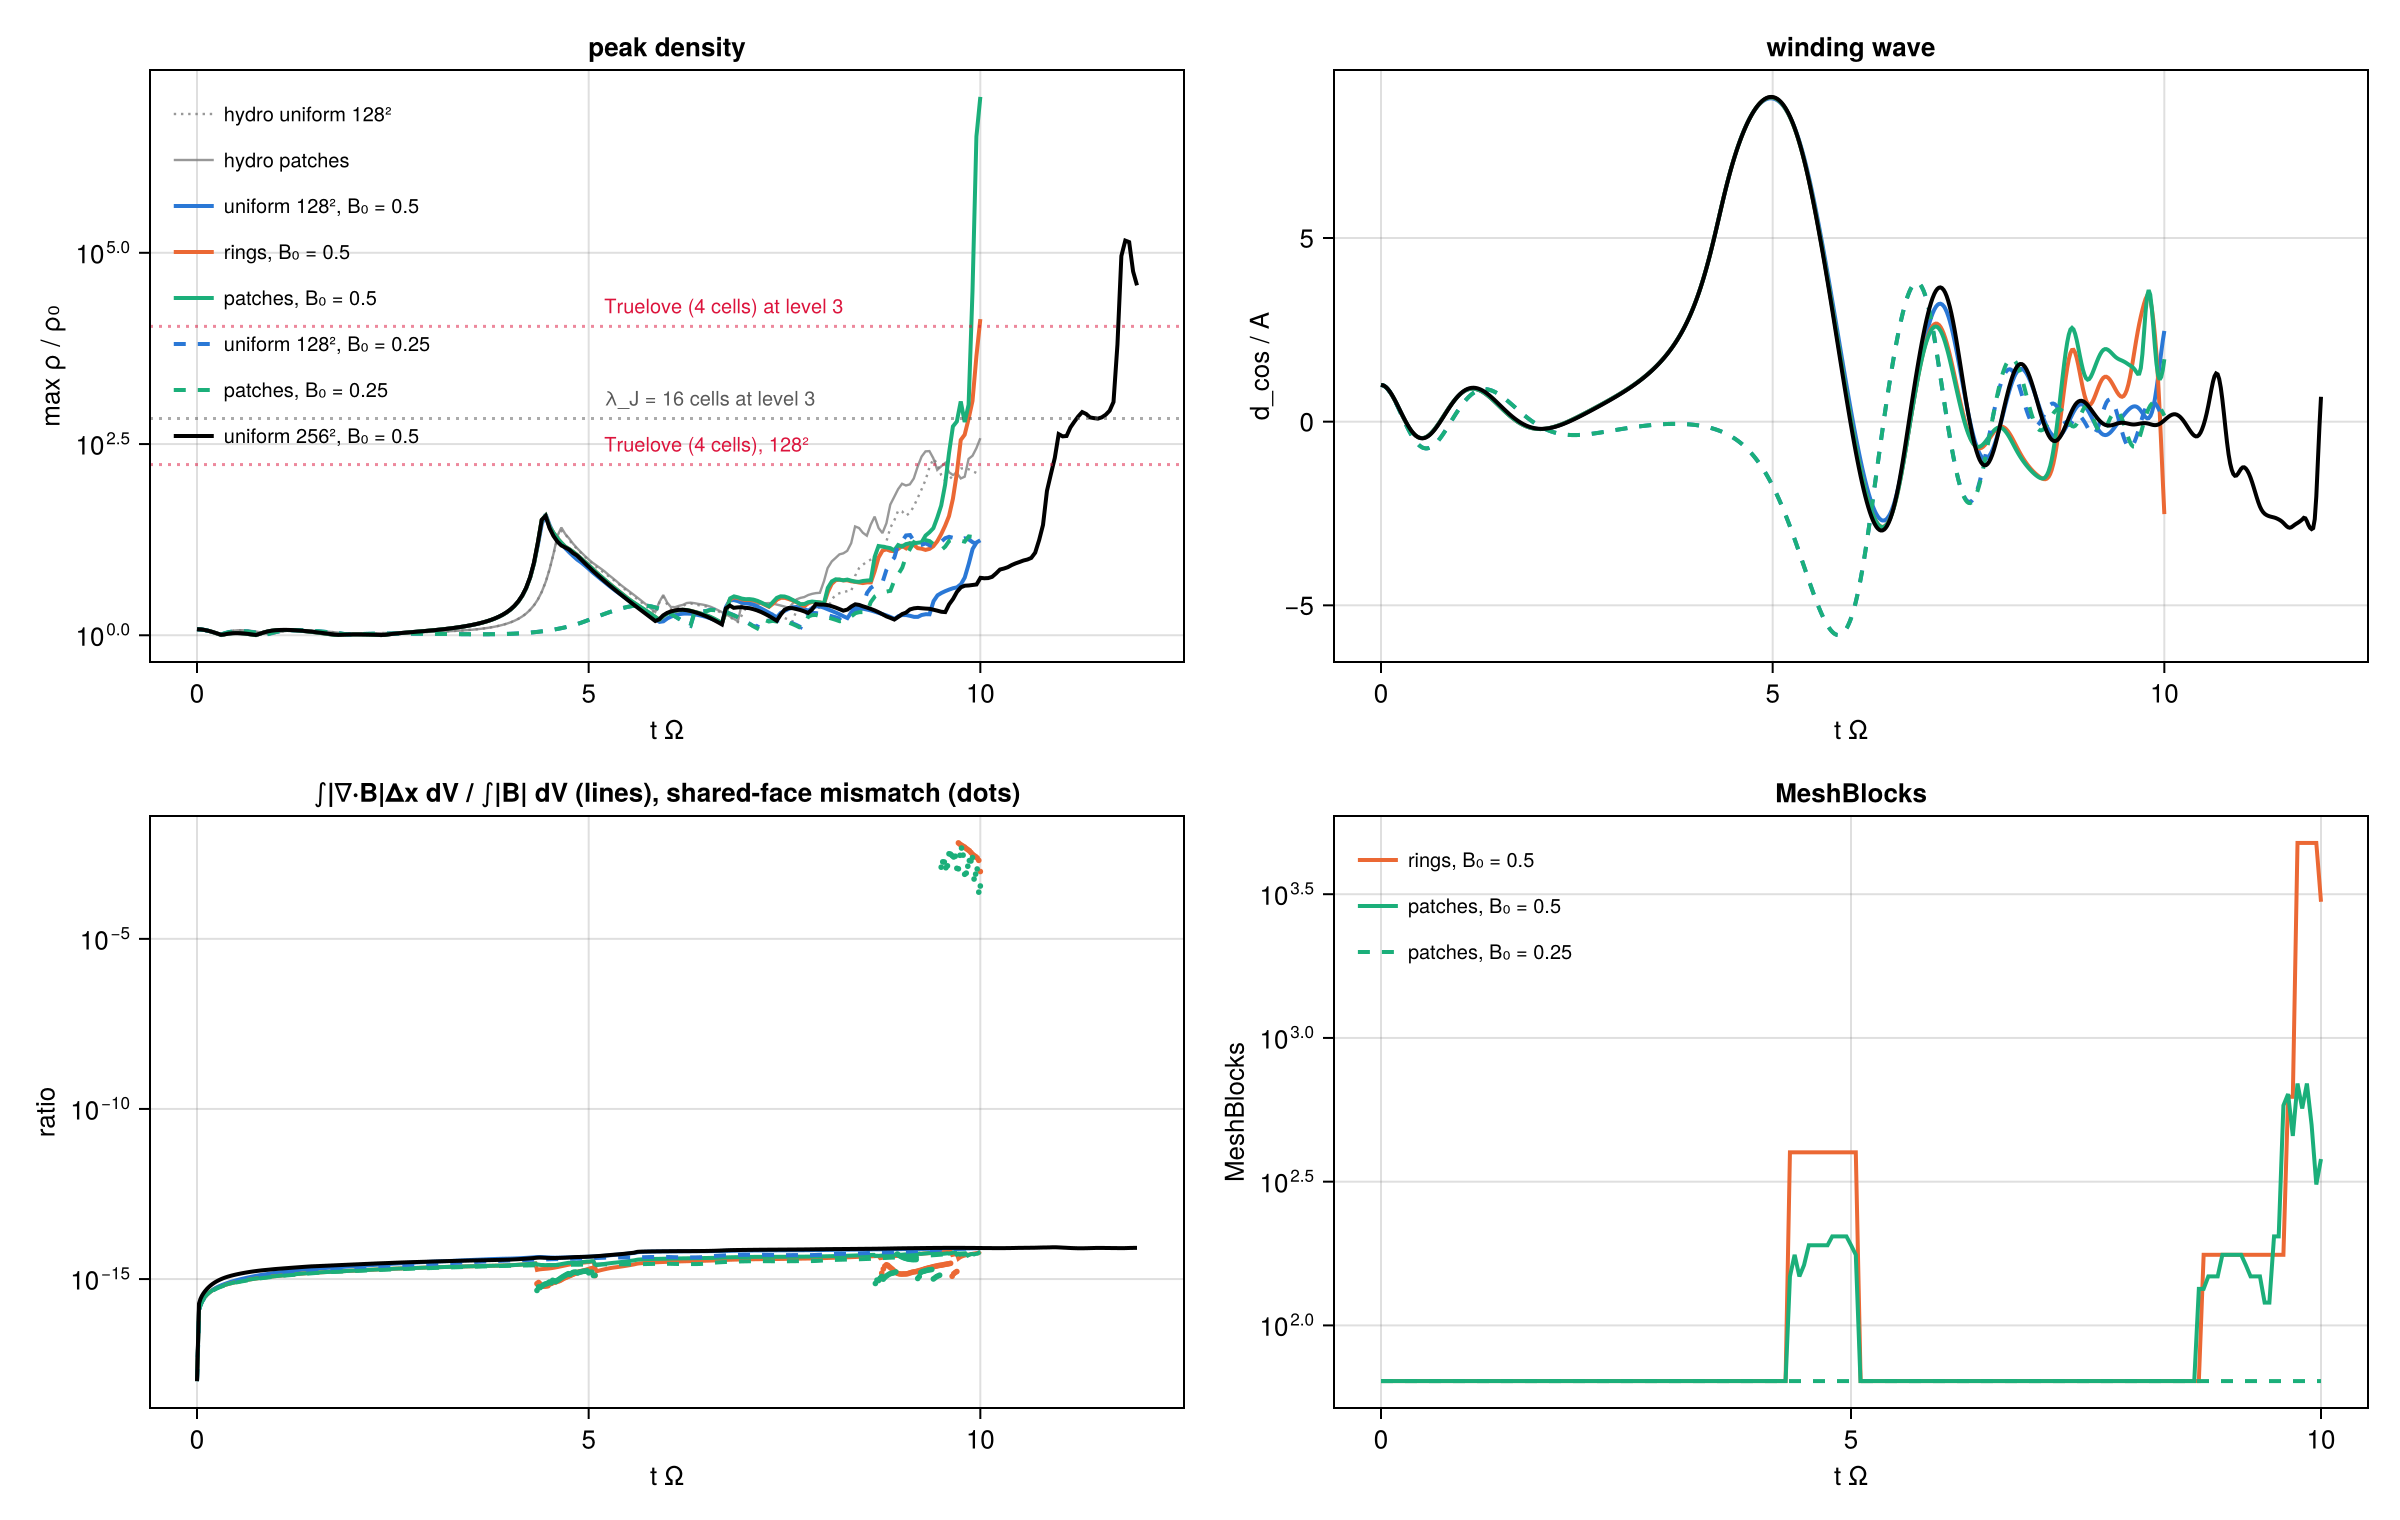
\includegraphics[width=\textwidth]{figures/fargo_amr_clump_mhd.png}
  \caption{Nonlinear swing, MHD. Top: peak density (hydro runs in gray for reference) and
  winding-wave amplitude. Bottom left: $|\nabla\!\cdot\!B|$ (lines) and the shared-face
  mismatch (dots); the jump at $t \approx 9.5$ comes with level 2 (see text). Bottom right:
  MeshBlock count.}
  \label{fig:clump_mhd}
\end{figure}

\begin{figure}[htb]
  \centering
  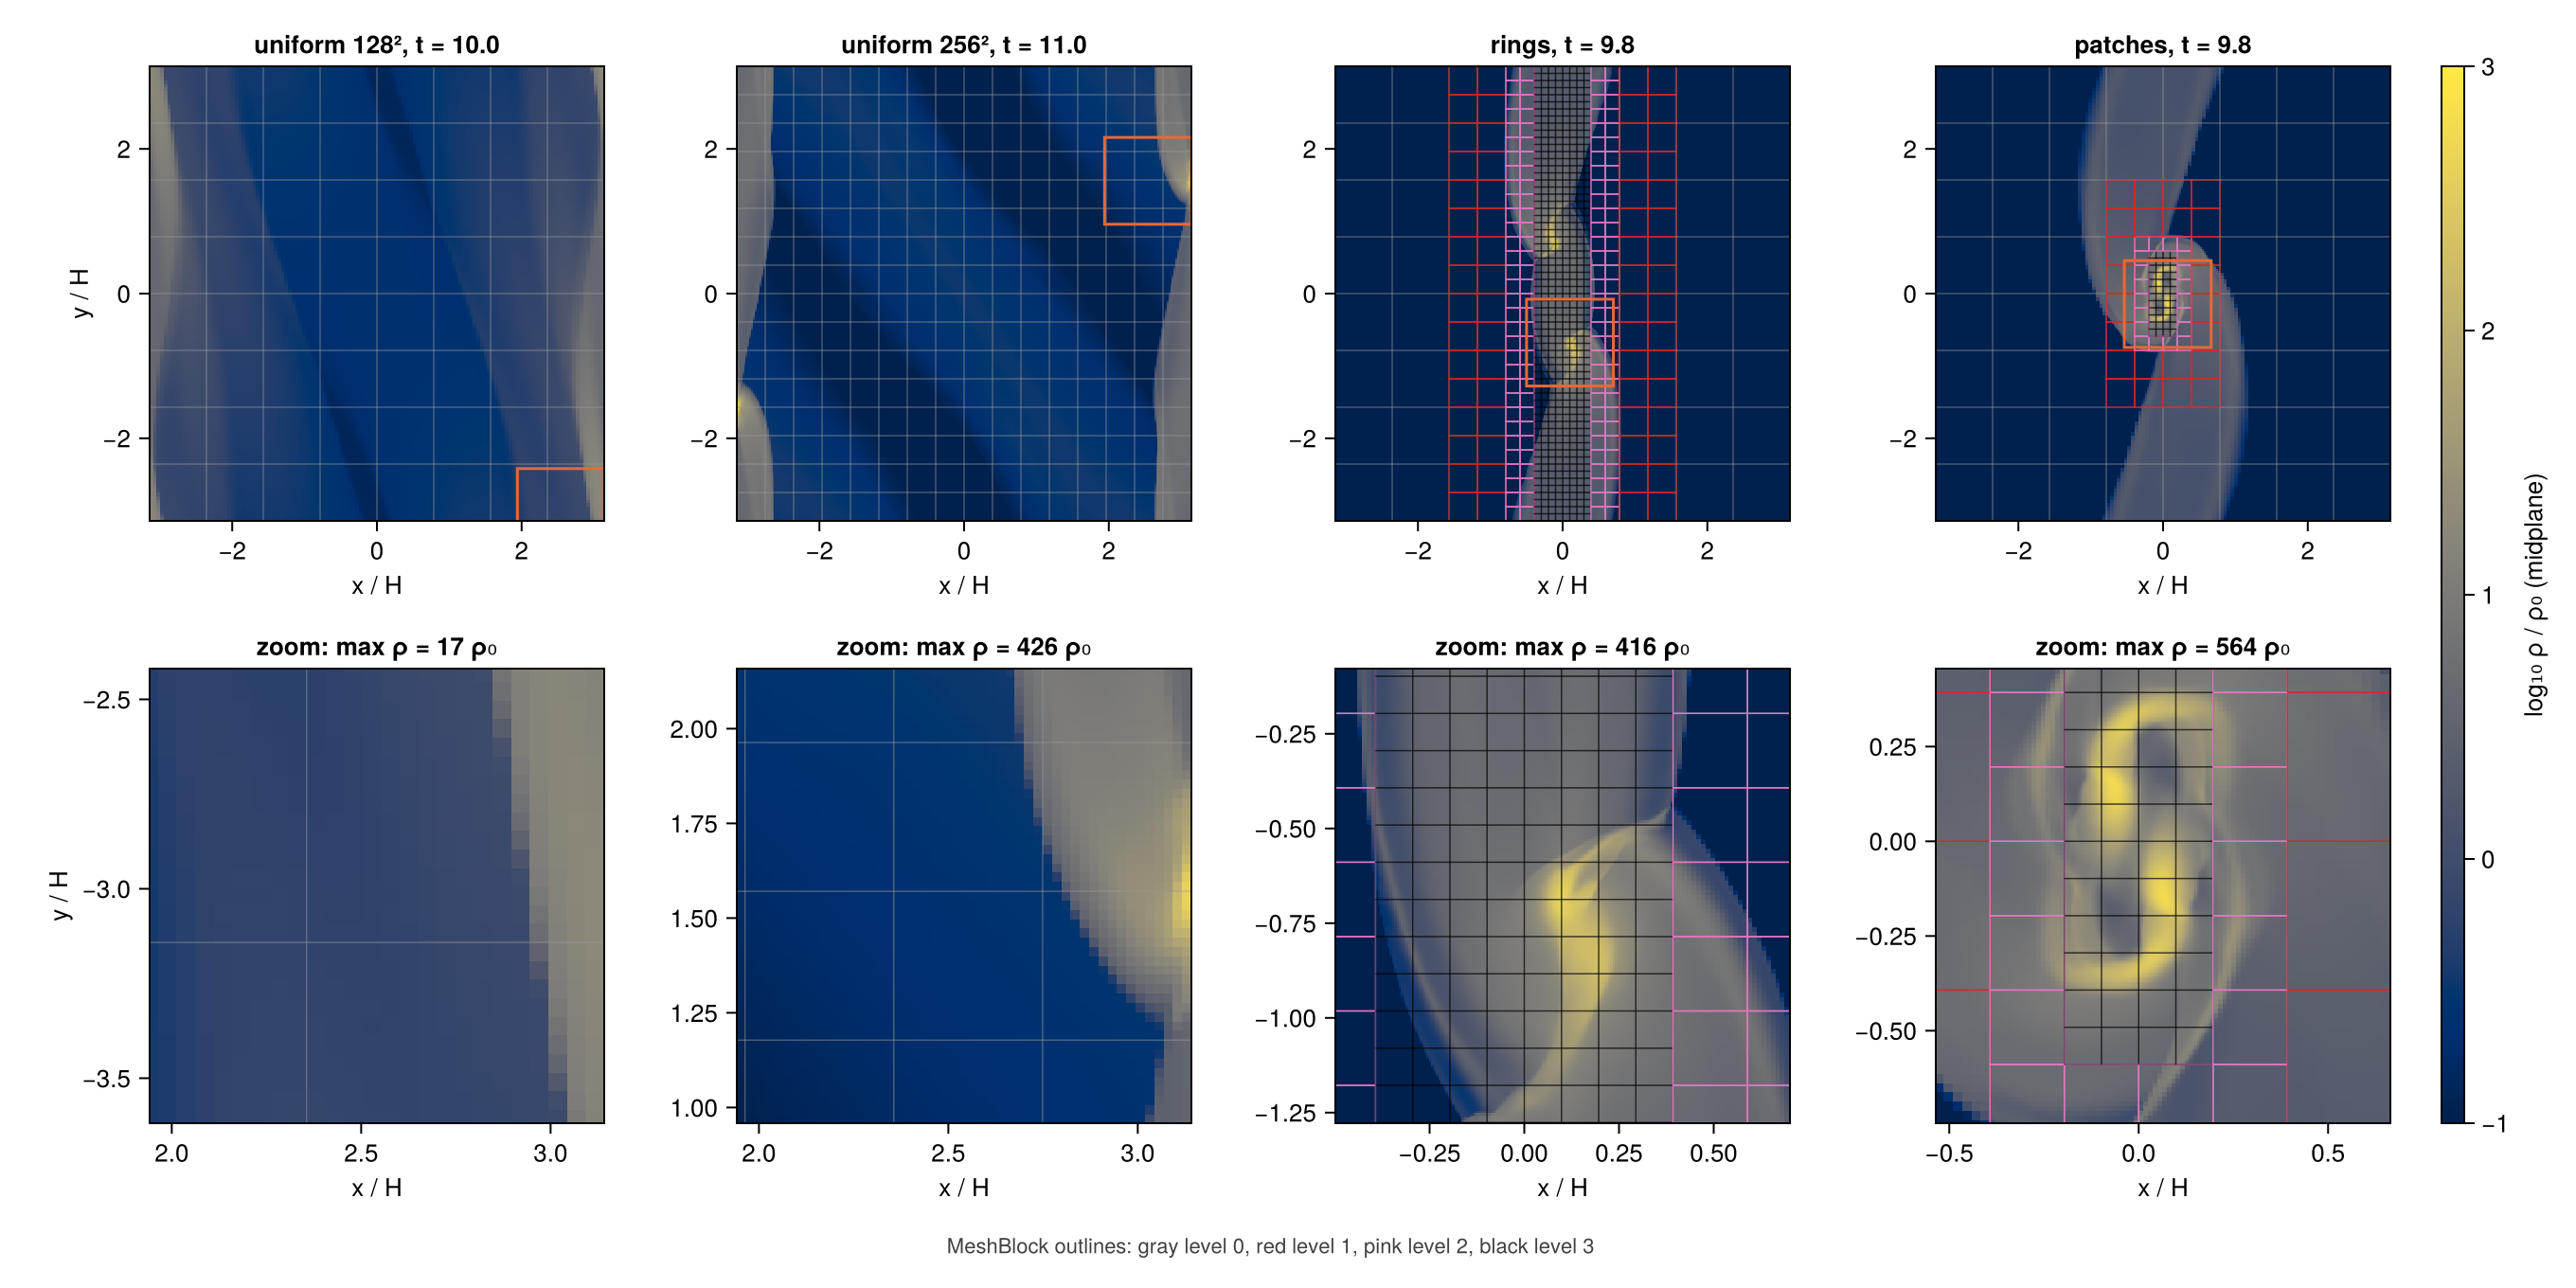
\includegraphics[width=\textwidth]{figures/fargo_amr_clump_mhd_maps.png}
  \caption{Midplane density of the $B_0 = 0.5$ runs, as Fig.~\ref{fig:clump_maps}: the
  refined runs at $t = 9.8$ and the uniform $256^2$ run at $t = 11$ (each near
  $400\rho_0$), the uniform $128^2$ run at $t = 10$. The uniform runs collapse on the
  shear-periodic $x_1$ boundary (the zooms stop at $x = \pi$), the refined runs at the
  centre.}
  \label{fig:clump_mhd_maps}
\end{figure}

%=========================================================================================
\section{Not yet validated}
\label{sec:open}
\begin{itemize}\itemsep2pt
\item \textbf{SC14 production.} The clump-following AMR of the gravito-turbulent box
      (\file{gravito\_turb\_l64z16\_clump\_amr\_overlay.athinput}) restarted from an
      archived $\beta = 3$ state, once with \code{oa\_annular = true} and once without:
      block count, cost per cycle and whether the timestep limit binds. Needs a cluster.
\item \textbf{$\nabla\!\cdot\!B$ at AMR derefinement} next to fine $x_2$ neighbours
      (\S\ref{sec:mhdB}): pre-existing in AthenaK, $10^{-13}$--$10^{-12}$ per event,
      to be fixed separately. Production MHD runs with box-shaped AMR should watch the
      history's \code{divb}.
\item \textbf{Face fields at AMR regrids with two or more levels} (\S\ref{sec:clump}):
      shared faces differ by $10^{-7}$--$10^{-3}$ after regrids, with or without orbital
      advection; reproducer in \file{run/fargo\_amr/mhd/twolev}. Probably the same root as
      the derefinement $\nabla\!\cdot\!B$ jumps.
\item \textbf{Converged collapse.} Refined runs collapse 1--1.3 time units before the
      uniform $256^2$ runs, hydro and MHD; a finer root grid or a criterion that refines
      the crests is needed, and a $512^2$ run to check $256^2$.
\item \textbf{Refinement on the shear-periodic $x_1$ boundary} (invariant I1). The $256^2$
      MHD clump forms there, out of reach of the refined runs.
\item \textbf{Non-FARGO refinement with $x_2$ level jumps} fails in the parent code
      (\S\ref{sec:shwave}); not addressed here.
\end{itemize}

%=========================================================================================
\section{Reproduction}
\label{sec:repro}
\begin{lstlisting}
cd validation/run/fargo_amr        # README.md: one command per run directory
python3 compare.py unif128 unif ring ypatch amrring amrbox   # shwave table
python3 errmap.py 00010                                      # error at the level jumps
(cd swing && python3 cmp.py)                                 # swing table
python3 ../swing_mhd_repro/repro.py 6 base fargo fargo_nofc  # MHD reproducer pairs
cd ../.. && julia figures/plot_fargo_amr_shwave.jl           # Fig. 2
julia figures/plot_fargo_amr_tests.jl                        # Figs. 1 and 3
julia figures/plot_fargo_amr_mhd.jl                          # Figs. 4, 5
julia figures/plot_fargo_amr_clump.jl     # nonlinear swing (run/fargo_amr/clump; README)
\end{lstlisting}


%=========================================================================================
\appendix
\section{Linear theory of the swing tests}
\label{app:theory}
The linear swing tests of \S\ref{sec:swing} and \S\ref{sec:mhd} (Figs.~\ref{fig:swing}
and~\ref{fig:mhd}) are compared with the amplitude equations of a single shearing wave in a
self-gravitating, magnetized shearing sheet. This appendix derives them, states the form
the code solves (the discrete Laplacian), and lists the checks. The equations are those of
the problem generator's header (\file{src/pgen/tests/swing.cpp}) and are integrated by
\file{validation/run/swing\_mhd/swing\_ode.py}.

\subsection{Background}
Local Cartesian coordinates rotating at $\Om$: $x$ radial, $y$ azimuthal, $z$ vertical.
The equilibrium is a uniform density $\rho_0$, pressure $p_0$, the shear flow
$\mathbf v_0 = -q\Om x\,\hat{\mathbf y}$ (with $q = 3/2$ for Keplerian rotation, epicyclic
frequency $\kappa^2 = 2(2-q)\Om^2$), and a uniform azimuthal field
$\mathbf B_0 = B_0\hat{\mathbf y}$. Units are Heaviside--Lorentz, as in AthenaK: the
magnetic pressure is $B^2/2$ and the Alfv\'en speed $v_A = B_0/\rho_0^{1/2}$. The field is
in equilibrium with the shear, since $\mathbf v_0\times\mathbf B_0 = 0$, and the tidal
force balances the Coriolis force of $\mathbf v_0$. The uniform background has no
self-gravity of its own (the Jeans swindle; in the periodic box the mean density does not
source the potential).

The equations are
\begin{align}
  &\partial_t\rho + \nabla\cdot(\rho\mathbf v) = 0, \\
  &\partial_t\mathbf v + (\mathbf v\cdot\nabla)\mathbf v =
    -\frac{\nabla p}{\rho} - \nabla\Phi
    + \frac{(\nabla\times\mathbf B)\times\mathbf B}{\rho}
    - 2\Om\hat{\mathbf z}\times\mathbf v + 2q\Om^2 x\,\hat{\mathbf x}, \\
  &\partial_t\mathbf B = \nabla\times(\mathbf v\times\mathbf B), \qquad
    \nabla^2\Phi = 4\pi G(\rho - \rho_0).
\end{align}
The perturbations are isentropic, $\delta p = c_s^2\,\delta\rho$: isothermal runs use the
isothermal sound speed, ideal-gas runs $c_s^2 = \gamma p_0/\rho_0$, with the initial
pressure perturbation set to match. All the linear tests here use $c_s = 1$.

\subsection{Linearized equations}
Write $\rho = \rho_0 + \delta\rho$, $\mathbf v = \mathbf v_0 + \mathbf u$,
$\mathbf B = \mathbf B_0 + \mathbf b$, $\Phi = \delta\Phi$, and restrict to
perturbations independent of $z$ with $u_z = b_z = 0$ (they stay zero: nothing couples to
them at $k_z = 0$). With the Lagrangian derivative of the shear flow
$\mathcal D \equiv \partial_t - q\Om x\,\partial_y$ and the terms
$(\mathbf u\cdot\nabla)\mathbf v_0 = -q\Om u_x\hat{\mathbf y}$ and
$-2\Om\hat{\mathbf z}\times\mathbf u = (2\Om u_y, -2\Om u_x)$:
\begin{align}
  \mathcal D\frac{\delta\rho}{\rho_0} &= -\nabla\cdot\mathbf u, \\
  \mathcal D u_x &= 2\Om u_y - c_s^2\partial_x\frac{\delta\rho}{\rho_0} - \partial_x\delta\Phi
     + \frac{B_0}{\rho_0}\left(\partial_y b_x - \partial_x b_y\right), \\
  \mathcal D u_y &= -(2-q)\Om u_x - c_s^2\partial_y\frac{\delta\rho}{\rho_0}
     - \partial_y\delta\Phi .
\end{align}
The Lorentz force is linearized as
$[(\mathbf B_0\cdot\nabla)\mathbf b - \nabla(\mathbf B_0\cdot\mathbf b)]/\rho_0$; its
$y$ component, $B_0(\partial_y b_y - \partial_y b_y)/\rho_0$, vanishes: a field along $y$
exerts no force along itself at $k_z = 0$. For the induction equation, with
$\nabla\times(\mathbf a\times\mathbf c) = \mathbf a(\nabla\cdot\mathbf c)
- \mathbf c(\nabla\cdot\mathbf a) + (\mathbf c\cdot\nabla)\mathbf a
- (\mathbf a\cdot\nabla)\mathbf c$,
\begin{align}
  \nabla\times(\mathbf v_0\times\mathbf b) &= (\mathbf b\cdot\nabla)\mathbf v_0
     - (\mathbf v_0\cdot\nabla)\mathbf b = -q\Om b_x\hat{\mathbf y} + q\Om x\,\partial_y\mathbf b, \\
  \nabla\times(\mathbf u\times\mathbf B_0) &= B_0\,\partial_y\mathbf u
     - B_0(\nabla\cdot\mathbf u)\,\hat{\mathbf y},
\end{align}
so that
\begin{equation}
  \mathcal D b_x = B_0\,\partial_y u_x, \qquad
  \mathcal D b_y = -q\Om b_x - B_0\,\partial_x u_x .
\end{equation}
The first term of the $b_y$ equation is the shear stretching radial field into azimuthal
field; the second, compression of the azimuthal field by radial motion.

\subsection{Shearing waves}
The coefficients depend on $x$ only through $\mathcal D$, so the equations admit shearing
waves (Kelvin modes) with a time-dependent radial wavenumber,
\begin{equation}
  \theta = k_x(t)\,x + k_y y, \qquad k_x(t) = k_{x0} + q\Om k_y t .
\end{equation}
Acting on $f(t)\,e^{i\theta}$, $\partial_t$ gives $\dot f + i\dot k_x x f$ and
$-q\Om x\partial_y$ gives $-iq\Om k_y x f$; the two cancel, so $\mathcal D$ becomes the
time derivative of the amplitude. A wave with $k_{x0} < 0$ is leading; the shear winds it
through $k_x = 0$ at $t = -k_{x0}/(q\Om k_y)$ (here $t = 4$ for $k_{x0} = -6$, $k_y = 1$)
into a trailing wave. In the shear-periodic box the wave is an exact solution for all $t$
when $k_{x0}$ and $k_y$ are box wavenumbers, because the boundary shift $q\Om L_x t$ in $y$
matches the change of $k_x$.

Take the phases of the initial condition (a density wave at rest):
\begin{equation}
  \frac{\delta\rho}{\rho_0} = \delta(t)\cos\theta, \quad
  \mathbf u = \mathbf w(t)\sin\theta, \quad
  \mathbf b = \mathbf c(t)\cos\theta, \quad
  \delta\Phi = \phi(t)\cos\theta .
\end{equation}
Then $\nabla\cdot\mathbf u = (k_x w_x + k_y w_y)\cos\theta$,
$\partial_x(\delta\rho/\rho_0) = -k_x\delta\sin\theta$,
$\partial_y b_x - \partial_x b_y = -(k_y c_x - k_x c_y)\sin\theta$ and
$\partial_y u_x = k_y w_x\cos\theta$, and the phases match term by term. The Poisson
equation gives $\phi = 4\pi G\rho_0\,\delta/D$ with $D = -k^2 = -(k_x^2 + k_y^2)$ in the
continuum. Collecting,
\begin{equation}
\boxed{
\begin{aligned}
  \dot\delta &= -(k_x w_x + k_y w_y), \\
  \dot w_x &= 2\Om w_y + k_x\Psi\,\delta - \frac{B_0}{\rho_0}\,(k_y c_x - k_x c_y), \\
  \dot w_y &= -(2-q)\Om w_x + k_y\Psi\,\delta, \\
  \dot c_x &= k_y B_0\, w_x, \\
  \dot c_y &= -k_x B_0\, w_x - q\Om c_x,
\end{aligned}
\qquad
\Psi(t) = c_s^2 + \frac{4\pi G\rho_0}{D(t)} ,}
\end{equation}
with $\delta(0) = A$ and $\mathbf w(0) = \mathbf c(0) = 0$. $\Psi$ is the effective
pressure: gravity lowers it, and it turns negative (the wave is Jeans unstable) while
$k^2 < 4\pi G\rho_0/c_s^2$, i.e.\ near $k_x = 0$ when $k_y^2 < 4\pi G\rho_0/c_s^2$. That
window, together with the epicyclic and shear terms, gives the transient swing
amplification (Goldreich \& Lynden-Bell 1965; Julian \& Toomre 1966; Toomre 1981; the
magnetized geometry is that of Kim \& Ostriker 2001). The system is linear, so the
amplitudes scale with $A$, and the figures plot $\delta/A$ and $c_y/A$.

\subsection{The discrete Laplacian}
The multigrid solver inverts the 7-point Laplacian, whose eigenvalue for $e^{i\theta}$ on
a grid of spacing $\Delta x = \Delta y$ is
\begin{equation}
  D_h = -\left(\frac{2}{\Delta x}\right)^2
        \left[\sin^2\frac{k_x\Delta x}{2} + \sin^2\frac{k_y\Delta y}{2}\right]
\end{equation}
($k_z = 0$ removes the third term), which tends to $-k^2$ as $k\Delta x \to 0$. The
comparisons use $D_h$ at the root spacing ($\Delta x = 2\pi/128$), the grid on which most
of the wave lives in the refined runs. With $4\pi G\rho_0 = 1.9$, $k_{x0} = -6$,
$k_y = 1$ the difference is small:

\begin{center}
\small
\begin{tabular}{@{}lccc@{}}
\toprule
$B_0$ & peak $\delta/A$ (time), continuum & the same, $D_h$ at $128^2$ & $\max_{t\le6}|c_y|/A$ \\
\midrule
0   & $-3.6090$ (7.811) & $-3.6083$ (7.812) & --- \\
0.5 & $+2.2938$ (7.117) & $+2.2994$ (7.117) & 1.566 \\
1.0 & $-2.8454$ (7.523) & $-2.8469$ (7.523) & 1.997 / 1.998 \\
\bottomrule
\end{tabular}
\end{center}

\noindent
(Peak over $t \le 8$.) The field reduces the amplification: magnetic pressure stiffens the
compression ($\Psi$ is effectively raised by $v_A^2$ for radial motions, see below), and
the azimuthal field carries the oscillation past the swing (Fig.~\ref{fig:mhd}).

\subsection{Checks}
\paragraph{Divergence.} $\nabla\cdot\mathbf b = -(k_x c_x + k_y c_y)\sin\theta$, and
\[
  \frac{d}{dt}(k_x c_x + k_y c_y) = q\Om k_y c_x + k_x k_y B_0 w_x
     + k_y(-k_x B_0 w_x - q\Om c_x) = 0,
\]
so a divergence-free initial field stays divergence-free; the integrator keeps
$k_x c_x + k_y c_y$ at $10^{-11}$ of $A$.

\paragraph{Axisymmetric limit.} For $k_y = 0$, $k_x$ is constant, $c_x$ stays zero, and the
system closes on $w_x$:
\[
  \ddot w_x = -\left[\kappa^2 + k_x^2\left(c_s^2 + v_A^2\right) - 4\pi G\rho_0\right] w_x ,
\]
the dispersion relation of axisymmetric magnetosonic--epicyclic waves in a
self-gravitating slab, $\omega^2 = \kappa^2 + k_x^2(c_s^2 + v_A^2) - 4\pi G\rho_0$ (with
$D = -k_x^2$): the field adds its pressure to the gas pressure for compressions
perpendicular to it.

\paragraph{Hydrodynamic limit.} For $B_0 = 0$ the field decouples ($\mathbf c$ is driven
only through $B_0$) and the first three equations are the self-gravitating hydrodynamic
swing of \S\ref{sec:swing}. Its peak is $-3.609$ at $t = 7.811$; at $t = 7.804$, the
output time at which the runs peak, it is $-3.605$, the value quoted there.

\subsection{Projections and the comparison}
The history output (\file{swing.cpp}) projects the solution on the instantaneous wave,
\[
  \texttt{d\_cos} = \frac{2}{V}\!\int\!\left(\frac{\rho}{\rho_0} - 1\right)\cos\theta\,dV,
  \quad
  \texttt{vx\_sin} = \frac{2}{V}\!\int\! v_x\sin\theta\,dV,
  \quad
  \texttt{by\_cos} = \frac{2}{V}\!\int\! \delta B_y\cos\theta\,dV,
\]
and likewise \code{vy\_sin}, \code{bx\_cos}, with $\theta$ built from $k_x(t)$. For a single
linear wave these return $\delta$, $w_x$, $w_y$, $c_x$, $c_y$ exactly; the sine
projection of the density, \code{d\_sin}, should stay zero, and its size measures phase
errors. Without orbital advection $v_y$ includes the shear flow, whose projection vanishes
($\int x\sin\theta\,dV = 0$ over a box with $k_y \neq 0$), so the same projections serve
both frames. The tables report, for a variable $f$ (here $\delta$ or $c_y$), the
trajectory deviation $\max_t|f - f_{\rm ref}|/\max_t|f_{\rm ref}|$ over the stated
interval, against linear theory (amplitude-scaled) or against the uniform twin
interpolated to common times. The integration uses an eighth-order Runge--Kutta
method (DOP853) with relative tolerance $10^{-11}$, so the theory curves are exact to
plotting precision.

\end{document}
